\setcounter{chapter}{4}
\setcounter{section}{0}
\part{RESULTADOS Y DISCUSIÓN} 

\section{Resultados de la metodología}

Los resultados que se obtuvieron al aplicar la metodología basada en el manifiesto del desarrollo ágil de software se redactan a continuación:

\subsection{Análisis de requisitos y obtención de pruebas}

Para llevar a cabo el análisis de los requisitos sobre la librería JavaScript que se desarrolló se tomaron en cuenta varios favores observando las carencias que existen al momento de realizar el modelamiento de cualquier software. Mediante el docente encargado de impartir las clases sobre cómo utilizar los lenguajes de modelado como lo es UML se dio cuenta que podría existir una forma en generar uno de los diagramas más importantes que es el diagrama de clases, pero a partir de las descripciones que se generan en los casos de uso del sistema.

La herramienta TDDT4IoTS permite realizar el modelamiento  preliminar de un software. La herramienta cuenta con SymLen para escribir las descripciones de casos de uso con datos técnicos sobre los objetos que intervendrán en el sistema informático que llevara a cabo la ejecución de todos los escenarios que se están describiendo. A petición del cliente recomendó que visitemos el sitio web de \url{aplicaciones.uteq.edu.ec/tddt4iots} para visualizar  los símbolos que usa la herramienta (ver ilustración \ref{fig:simbolostdd}).

\begin{figure}[H]
	\centering
	\caption{Símbolos que utiliza la herramienta TDDT4IoTS}
	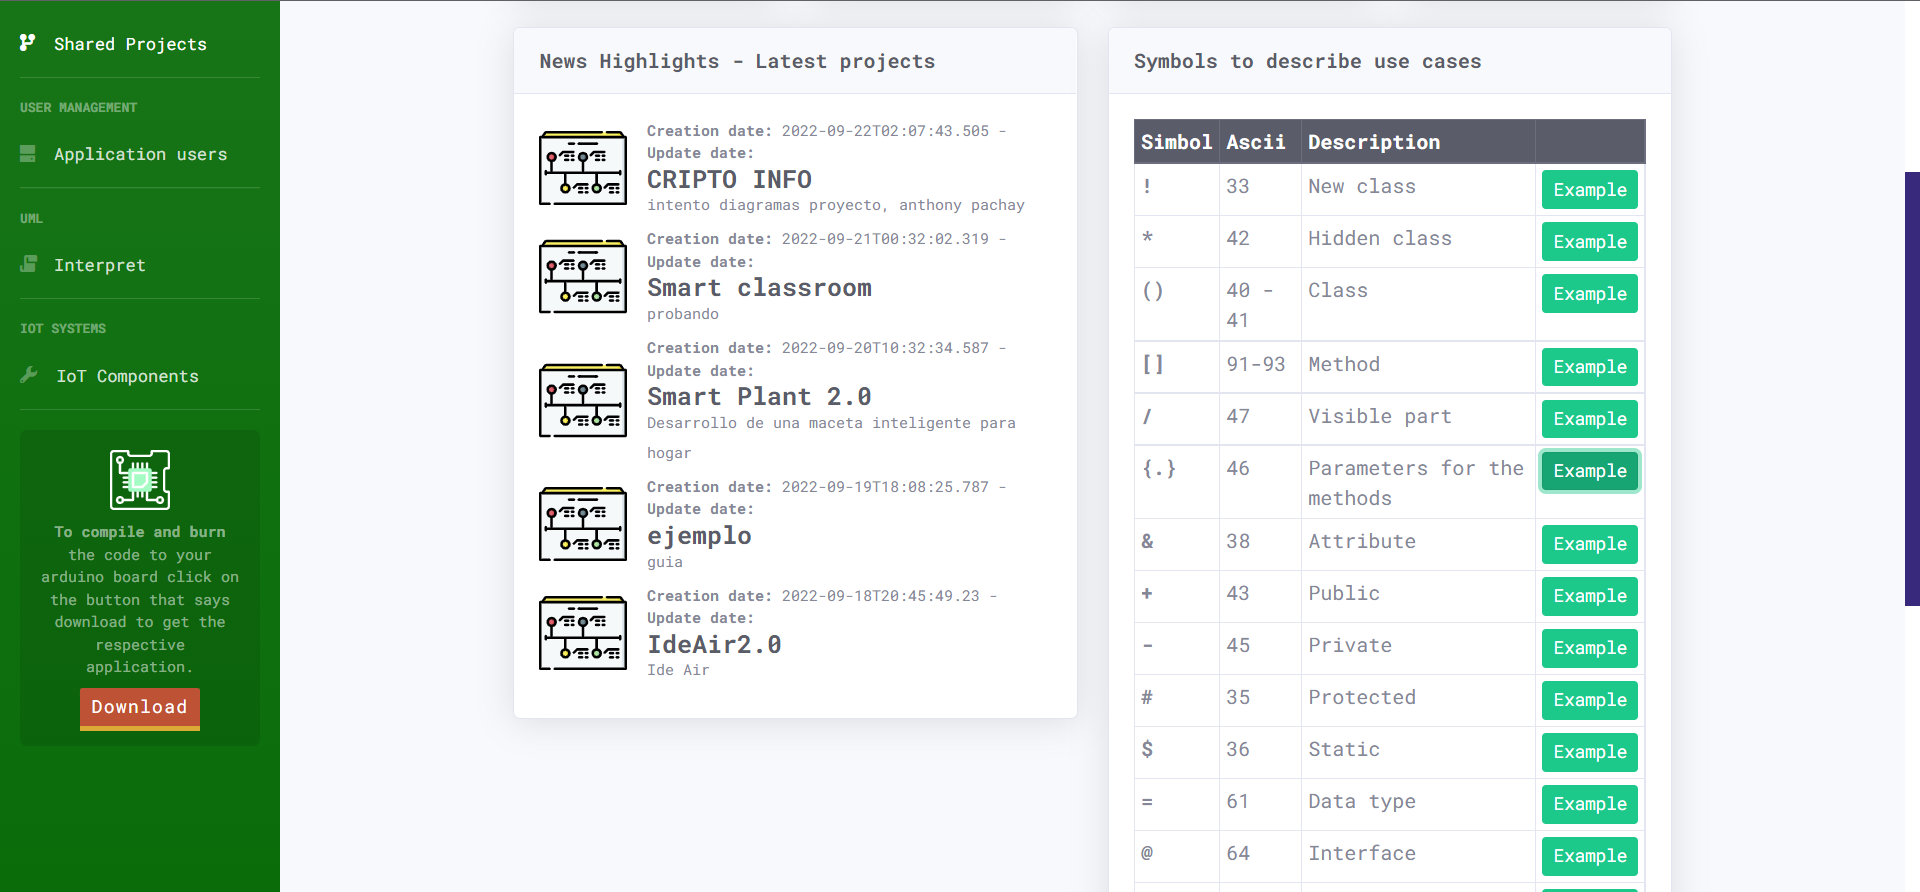
\includegraphics[width=12cm]{img/res_001.png}
	\label{fig:simbolostdd}
	\vspace{4mm}
	{\footnotesize \textbf{\\ FUENTE: INVESTIGACIÓN} \textbf{\\ ELABORADO: AUTOR}}
\end{figure}

En la lista de símbolos que se visualiza en la ilustración anterior se encuentra un botón que dice \textit{"Example"}. Si presionamos en ese botón se pudo observar un ejemplo detallado sobre cómo se deben utilizar los símbolos para tratar de especificar algún objeto del diagrama de clases que se genera mediante la descripción del caso de uso pertinente (ver ilustracións \ref{fig:ejemploclase}, \ref{fig:ejemploparametro}).

\begin{figure}[H]
	\centering
	\caption{Ejemplo de cómo se debe utilizar el símbolo respectivo para crear una clase.}
	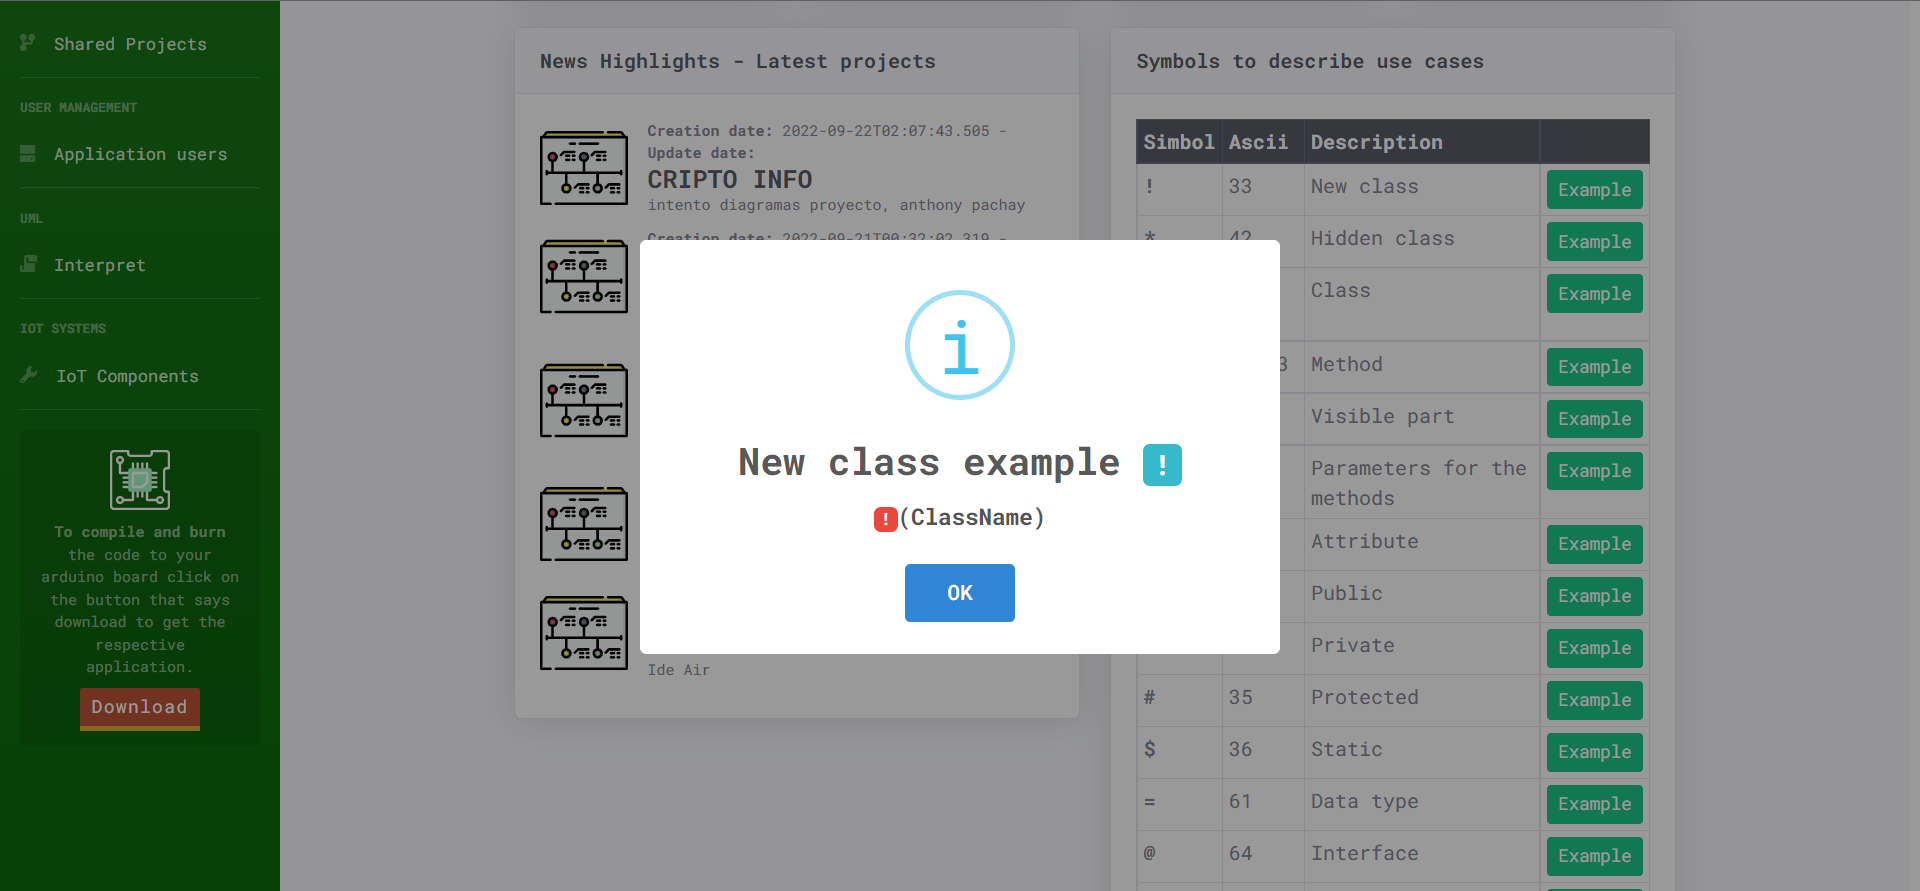
\includegraphics[width=14cm]{img/res_002.png}
	\label{fig:ejemploclase}
	\vspace{4mm}
	{\footnotesize \textbf{\\ FUENTE: INVESTIGACIÓN} \textbf{\\ ELABORADO: AUTOR}}
\end{figure}

\begin{figure}[H]
	\centering
	\caption{Ejemplo de cómo se debe utilizar el símbolo respectivo generar los parámetros de un método declarado con el lenguaje de símbolos.}
	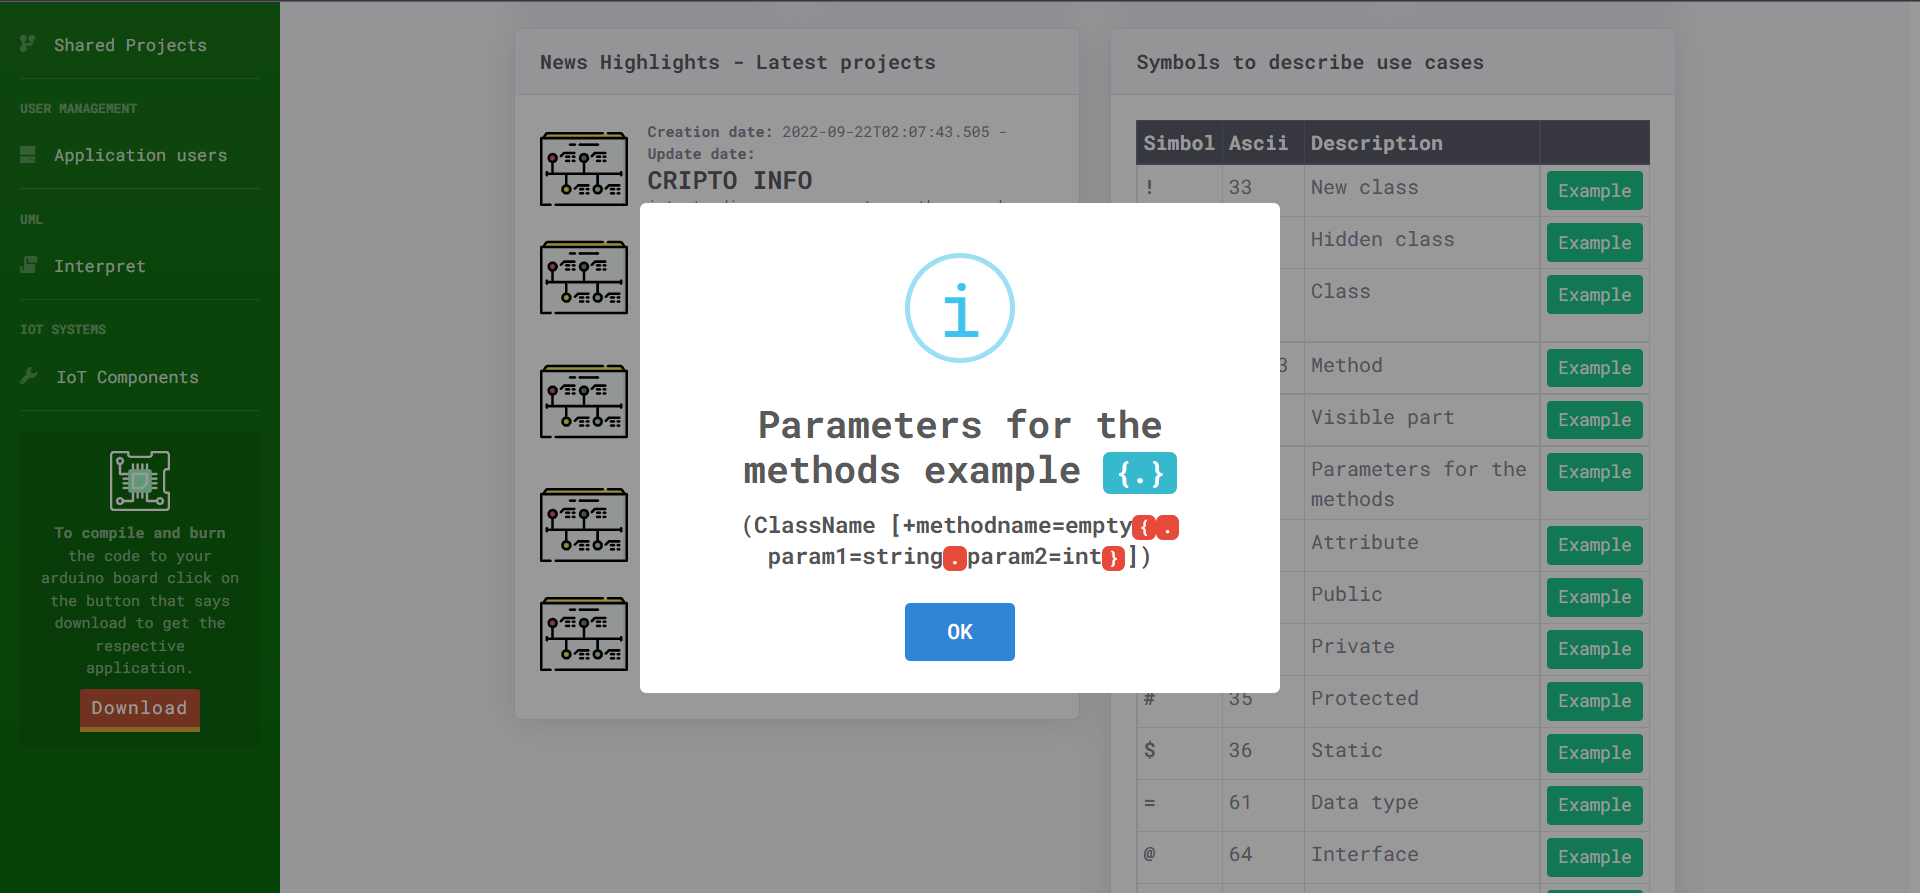
\includegraphics[width=14cm]{img/res_003.png}
	\label{fig:ejemploparametro}
	\vspace{4mm}
	{\footnotesize \textbf{\\ FUENTE: INVESTIGACIÓN} \textbf{\\ ELABORADO: AUTOR}}
\end{figure}

Luego de tener una idea general sobre los símbolos que utiliza la herramienta se especificaron detalladamente los significados de cada símbolo y como puede ser utilizado en las descripciones de los casos de uso. 

\sloppy
\begin{itemize}
	\item \textbf{Asterisco *}: Este símbolo sirve para ocultar cualquier carácter que se encuentre redactado después de el mismo. Esto permitirá al momento de interpretar la descripción del caso de uso ingresada eliminar los caracteres mezclados con los símbolos y solo dejar visibles los caracteres normales formando un texto natural que pueda ser entendido por cualquier persona regular. \textbf{Ejemplo:}
	
	\begin{verbatim}
		* texto de prueba
	\end{verbatim}
	
	\item \textbf{Paréntesis de apertura y cierre ()}: Este símbolo sirve para especificar uno de los componentes más importantes del diagrama de clases, dentro de los paréntesis de apertura y cierra se deberá especificar el nombre de la clase u objeto que se pretende generar de forma automática. Cabe mencionar que, si se escribe el nombre de clase separada por espacios, la librería deberá omitir estos espacios y auto completarlos con la segunda letra después del espacio con mayúscula. \textbf{Ejemplo:}  
	
	\begin{verbatim}
		(Nombre de la clase)
	\end{verbatim}
	
	\item \textbf{Corchete de apertura y cierre []:} Este símbolo podrá ser utilizado dentro de los símbolos para crear las clases, permitirá definir Los métodos o funciones que pertenecerá a la clase respectiva. \textbf{Ejemplo:}
	
	\begin{verbatim}
		(Nombre de la clase [+nombre del método=empty])
	\end{verbatim} 
	
	\item \textbf{Slash /:} Este símbolo es bastante interesante, con él se deben visualizar  caracteres que se encuentre encerrado de un slash de apertura y otro slash de cierre. Este símbolo se lo deberá usar cuando todos los caracteres se encuentren después del símbolo del asterisco, la idea es permitir que se visualicen caracteres específicos dentro de los datos técnicos para generar el diagrama de clases, sin afectar el uso de los demás símbolos. \textbf{Ejemplo:}
	
	\begin{verbatim}
		(Nombre de la clase &+/nombre/=string)
	\end{verbatim} 
	
	\item \textbf{Llaves de apertura y llaves de cierre con punto \{.\}:} Con el símbolo de las llaves se podrá definir los parámetros de entrada para los métodos o funciones de las clases. Cada parámetro estará separado por un punto, además se deberá utilizar el símbolo del igual (=) para especificar su tipo de dato. Cada recalcar que todos los atributos también deberán estar especificados dentro de las llaves de apertura y cierre. \textbf{Ejemplo:}
	
	\begin{verbatim}
		(Nombre de la clase [+nombre del método=empty
		{.param1=string.param2=strgin}])
	\end{verbatim}
	
	\item \textbf{Ampersand \&: } Este símbolo debe permitir declarar los atributos de la clase que fue creada con el símbolo anterior. Existen otros símbolos que interviene en la creación de otros componentes del diagrama de clases, más adelante se detallaran para que sirven. \textbf{Ejemplo:}
	
	\begin{verbatim}
		(Nombre de la clase &+atributo uno=string &+atributo 
		dos=string)
	\end{verbatim}
	
	\item \textbf{Visibilidad +: } El símbolo de suma permite especificar que la visibilidad del atributo, método o función será de manera pública. \textbf{Ejemplo:}
	
	En este ejemplo se visualiza la forma en cómo utilizar el símbolo de suma en atributos de clase.
	
	\begin{verbatim}
		(Nombre de la clase &+atributo uno=string &+atributo 
		dos=string)
	\end{verbatim}
	
	En este ejemplo se visualiza la forma en cómo utilizar el símbolo de suma en métodos o funciones de clase.
	
	\begin{verbatim}
		(Nombre de la clase [+nombre del método=empty
		{.param1=string.param2=strgin}])
	\end{verbatim}
	
	\item \textbf{Visibilidad -: } El símbolo de resta permite especificar que la visibilidad del atributo, método o función será de manera privada. \textbf{Ejemplo:}
	
	En este ejemplo se visualiza la forma en cómo utilizar el símbolo de suma en atributos de clase.
	
	\begin{verbatim}
		(Nombre de la clase &-atributo uno=string &-atributo 
		dos=string)
	\end{verbatim}
	
	En este ejemplo se visualiza la forma en cómo utilizar el símbolo de suma en métodos o funciones de clase.
	
	\begin{verbatim}
		(Nombre de la clase [-nombre del método=empty
		{.param1=string.param2=strgin}])
	\end{verbatim}
	
	\item \textbf{Visibilidad \#: } El símbolo de almohadilla permite especificar que la visibilidad del atributo, método o función será de manera protegida. \textbf{Ejemplo:}
	
	En este ejemplo se visualiza la forma en cómo utilizar el símbolo de suma en atributos de clase.
	
	\begin{verbatim}
		(Nombre de la clase &#atributo uno=string &#atributo 
		dos=string)
	\end{verbatim}
	
	En este ejemplo se visualiza la forma en cómo utilizar el símbolo de suma en métodos o funciones de clase.
	
	\begin{verbatim}
		(Nombre de la clase [#nombre del método=empty
		{.param1=string.param2=strgin}])
	\end{verbatim}
	
	\item \textbf{Visibilidad \$: } El símbolo de dólar permite especificar que la visibilidad del atributo, método o función será de manera estática. \textbf{Ejemplo:}
	
	En este ejemplo se visualiza la forma en cómo utilizar el símbolo de suma en atributos de clase.
	
	\begin{verbatim}
		(Nombre de la clase &$atributo uno=string &$atributo 
		dos=string)
	\end{verbatim}
	
	En este ejemplo se visualiza la forma en cómo utilizar el símbolo de suma en métodos o funciones de clase.
	
	\begin{verbatim}
		(Nombre de la clase [$nombre del metodo=empty
		{.param1=string.param2=strgin}])
	\end{verbatim}
	
	\item \textbf{Igual =:} El símbolo de igual debe permitir asignar el tipo de dato a los atributos, métodos o funciones declaradas dentro de la clase. En el caso de los métodos de tipo \textbf{void}  se deberá utilizar la palabra \textit{empty} indiciando que es un método que retornara ningún valor. \textbf{Ejemplo:}
	
	\begin{verbatim}
		{.param1=string.param2=strging}
	\end{verbatim}
	
	\item \textbf{Arroba @:} El símbolo de arroba se lo utiliza dentro de los paréntesis que permiten generar una clase del diagrama. Pero se recuerda que en el diagrama de clases también se pueden crear interfaces. El objetivo de este símbolo es utilizarlo dentro de los paréntesis, pero el interprete identificara que sera una interfaz la que se deberá crear. \textbf{Ejemplo:}
	  
	\begin{verbatim}
		(@nombre interfaz)
	\end{verbatim}

	\item  \textbf{Signo de interrogación apertura y cierre ¿?:} El símbolo de interrogación se lo utiliza para generar otro tipo de objeto principal del diagrama de clases. El objetivo principal de este símbolo es generar los enum. \textbf{Ejemplo:}
	
	\begin{verbatim}
		¿enumTest?
	\end{verbatim}

	\item \textbf{Cierra comillas bajas »:} El símbolo  de cierre comillas bajas se lo utiliza para agregar atributos a un objeto principal del diagrama de clases. El objetivo principal de este símbolo es atributos dentro de los objetos enum. \textbf{Ejemplo:}
	
	\begin{verbatim}
		¿enumTest »atributoUno »atributoDos?
	\end{verbatim}

	\item \textbf{Porcentaje \%:} El símbolo de porcentaje sirve para agregar nuevos constructores a las clases que ya fueron definidas, además para especificar sus parámetros se utiliza los mismos símbolos para agregar atributos a la clase, con la diferencia que los parámetros van separados por la coma. \textbf{Ejemplo:}
	
	\begin{verbatim}
		*(class %.class=Class, .param=string%)
	\end{verbatim}
	  
\end{itemize}

Dentro del diagrama de clases existen diferentes tipos de relaciones con las que se pueden relacionar las clases que se encuentran definidas. Para implementar las relaciones también se utilizan una combinación de símbolos que permitan detectarlas y la librería se encarga de generarlas. A continuación, se especificarán los símbolos que se utilizan para los tipos de relaciones en el diagrama de clases:

\begin{itemize}
	\item \textbf{Símbolo de admiración de apertura ¡!:} Para indicar que se va realizar una relación entre 2 objetos del diagrama de clases, el texto debe estar entre este símbolo tanto en su apertura y cierre.
	
	\item \textbf{Corchete de apertura y cierre []:} Dentro del símbolo de admiración se podrá indicar un texto como leyenda sobre la línea de la relación, esto indicara alguna palabra clave sobre la relación entre los objetos.
	
	\item \textbf{Cardinalidad 1 o n:} Sobre la línea de la relación se puede indicar una cardinalidad de uno a muchos. El numero \textit{\underline{1}} indicará que la cardinalidad es de 1 y si usa la letra \textit{\underline{n}} indicará que la cardinalidad des de muchos. Se los debe utilizar en la parte exterior de los corchetes.
	
	\item \textbf{Agregación > >:} Para indicar que el tipo de relación entre dos objetos del diagrama de clases se utiliza los símbolos de \textit{> >}. Se deben colocar en la parte exterior donde se el texto de cardinalidad. \textbf{Ejemplo:}
	
	
	\begin{verbatim}
		*¡claseUno 1>[texto de cardinalidad]>n claseDos!
	\end{verbatim}

	\item \textbf{Dependencia < <:} Para indicar que el tipo de relación entre dos objetos del diagrama de clases se utiliza los símbolos de \textit{< <}. Se deben colocar en la parte exterior donde se el texto de cardinalidad. \textbf{Ejemplo:}
	
	\begin{verbatim}
		*¡claseUno 1<[texto de cardinalidad]<n claseDos!
	\end{verbatim}

	\item \textbf{Generalización < >:} Para indicar que el tipo de relación entre dos objetos del diagrama de clases se utiliza los símbolos de \textit{<>}. Se deben colocar en la parte exterior donde se el texto de cardinalidad. \textbf{Ejemplo:}
	
	\begin{verbatim}
		*¡claseUno 1<[texto de cardinalidad]>n claseDos!
	\end{verbatim}

	\item \textbf{Asociación > <:} Para indicar que el tipo de relación entre dos objetos del diagrama de clases se utiliza los símbolos de \textit{> <}. Se deben colocar en la parte exterior donde se el texto de cardinalidad. \textbf{Ejemplo:}
	
	\begin{verbatim}
		*¡claseUno 1>[texto de cardinalidad]<n claseDos!
	\end{verbatim}
	
\end{itemize}

En la tabla se describe el código ASCII para escribir los símbolos mediante el teclado de una computadora. Se pretendió que cada símbolo tenga una combinación ASCII para que el analista pueda escribir cada símbolo con el teclado y no obtenerlo de alguna forma que sea complicada.

\begin{table}[h!]
	\centering
	\caption{Código ASCII para cada símbolo del lenguaje.}
	\begin{tabular}{p{2cm}p{4cm}p{5cm}}
		\toprule
		\textbf{Símbolo} & \textbf{ASCII} & \textbf{Descripción} \\
		\midrule
		* & 33 & Ocultar texto \\
		\addlinespace
		( ) & 40 - 41 & Crear clase \\
		\addlinespace
		\textbf{[ ]} & 91 - 93 & Crear método \\
		\addlinespace
		/ & 47 & Parte visible \\
		\addlinespace
		\{.\} & 123 - 125	 & Parámetro de los métodos \\
		\addlinespace 	
		\& & 38 & Atributo de clase \\
		\addlinespace
		+ & 43 & Publico \\
		\addlinespace
		- & 45 & Privado \\
		\addlinespace
		\# & 35 & Protegido \\
		\addlinespace
		\$ & 36 & Estático \\
		\addlinespace
		= & 61 & Tipo de dato \\
		\addlinespace
		@ & 64 & Interfaz \\
		\addlinespace
		¿? & 168 - 63 & Enum \\
		\addlinespace
		\% & 37 & Constructores \\
		\addlinespace
		\bottomrule
	\end{tabular}
	\vspace{4mm}
	{\footnotesize \textbf{\\ FUENTE: INVESTIGACIÓN} \textbf{\\ ELABORADO: AUTOR}}
\end{table}

Para definir los diferentes tipos de relaciones que se usaran en el diagrama de clases. En la tabla se visualiza un grupo de símbolos que servirán para crear las relaciones de tipo: agregación, dependencia, herencia o generalización y asociación. 

\newpage

\begin{table}[h!]
	\centering
	\caption{Código ASCII para cada símbolo del lenguaje que especifican las relaciones.}
	\begin{tabular}{p{2cm}p{4cm}p{6cm}}
		\toprule
		\textbf{Símbolo} & \textbf{ASCII} & \textbf{Descripción} \\
		\midrule
		¡! & 33 - 173 & Crear relación \\
		\addlinespace
		\textbf{[ ]} & 91 - 93 & Especificar leyenda en la relación \\
		\addlinespace
		1[ ]1 & -- & Cardinalidad de uno a uno \\
		\addlinespace
		1[ ]n & -- & Cardinalidad de uno a muchos \\
		\addlinespace
		n[ ]1 & -- & Cardinalidad de muchos a uno \\
		\addlinespace
		> > & 62 - 62 & Agregación \\
		\addlinespace
		< < & 60 - 60 & Dependencia \\
		\addlinespace
		< > & 60 - 62 & Generalización \\
		\addlinespace
		> < & 62 - 60 & Asociación \\
		\addlinespace
		\bottomrule
	\end{tabular}
	\vspace{4mm}
	{\footnotesize \textbf{\\ FUENTE: INVESTIGACIÓN} \textbf{\\ ELABORADO: AUTOR}}
\end{table}

Luego de a ver recopilado todos los símbolos que la librería va a interpretar, el docente proporciono 1 caso de uso. Además, proporciono el gráfico del diagrama de clases que se escribió en los casos de uso. En la ilustración \ref{fig:usecasetest} se observa el caso de uso de prueba para saber que objetos debe generar la librería. 

\begin{figure}[h!]
	\centering
	\caption{Diagrama de casos de uso para las pruebas.}
	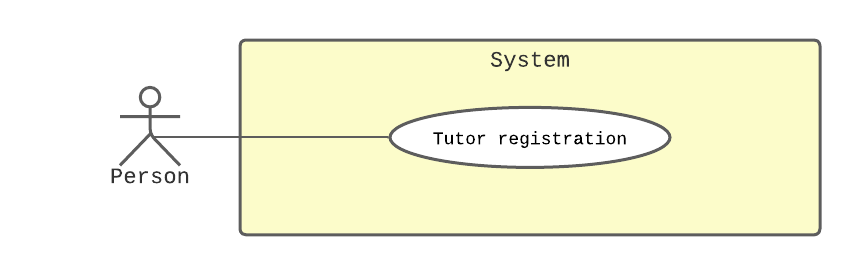
\includegraphics[width=13cm]{img/usecaseTest.png}
	\label{fig:usecasetest}
	\vspace{4mm}
	{\footnotesize \textbf{\\ FUENTE: INVESTIGACIÓN} \textbf{\\ ELABORADO: AUTOR}}
\end{figure}

Para comprender totalmente las acciones que se deben ejecutar en el caso de uso que se usara como prueba, está escrito en 2 distintas formas. En la tabla \ref{tab:usecasetutorregistration} se observa la descripción del caso de uso en lenguaje natural especificando todas las acciones con el objetivo que cualquier persona regular logre entender. En la tabla \ref{tab:usecasetutorregistration_symbol} se observa la misma descripción del caso de uso pero utilizando los símbolos.   

\begin{table}[h!]
	\centering
	\caption{Descripción del caso de uso Registrar tutor.}
	\label{tab:usecasetutorregistration}
	\begin{tabular}{| p{3cm} | p{11cm} |}
		\hline
		\textbf{Caso de uso:} & Registrar tutor \\ \hline
		\textbf{Actores:} & Persona \\ \hline
		\textbf{Poscondición:} & Usuario registrado en la base de datos. \\ \hline
		\textbf{Precondición:} & El usuario existe en la base de datos. \\ \hline
		\textbf{Propósito:} & Ingresar a la interfaz principal de la aplicación \\ \hline
		\textbf{Resumen:} & 
		Permite identificar las credenciales del usuario que intenta ingresar al sistema, de esa forma verificar el tipo de usuario que ingresa. \\ \hline
		\textbf{Tipo:} & Primario \\ \hline
		\multicolumn{2}{ |c| }{\textbf{Flujo normal}} \\ \hline
	\end{tabular}
\begin{tabular}{| p{7cm} | p{7cm} |}
	1. Este caso de uso comienza cuando una persona quiere registrarse como usuario tutor en el sistema.  & \\ \hline
	2. La persona accede entonces a la interfaz de registro de usuarios. & \\ \hline
	& 3. Le muestra los campos a rellenar en la interfaz de registro de usuarios: nombre, apellido, fecha de nacimiento, sexo, número de teléfono, correo electrónico, nombre de usuario contraseña. Hay que tener en cuenta que el registro de una Persona tiene un Usuario. Hay estados que pueden ser Desactivado o Activado que cada Usuario tendrá un Estado. También hay varios tipos de usuarios, que son Tutor o Paciente o Administrador y cada Usuario tendrá un Tipo de Usuario. Además, el sistema asigna un id cuando lo almacena. \\ \hline
	4.La persona introduce todos los datos requeridos por la vista, y hace clic en enviar. & \\ \hline
	& 5. Crear un objeto persona. \\ \hline
	& 6. Crear un objeto tutor. \\ \hline
	& 7. Crear un objeto de usuario. \\ \hline
	& 8. Guarda los datos del tutor en la base de datos. \\ \hline
	& 9. Guarda los datos del usuario en la base de datos. \\ \hline
	& 10. Este caso de uso termina cuando el sistema muestra la interfaz de inicio de sesión.  \\ \hline
		\end{tabular}
		\vspace{4mm}
	{\footnotesize \textbf{\\ FUENTE: INVESTIGACIÓN} \textbf{\\ ELABORADO: AUTOR}}
\end{table}


Para la elaboración de la descripción del caso de uso con los símbolos proporcionaron información de un diagrama de clases que ya se encontraba realizado. El objetivo de este caso de uso era escribir todas las acciones con información técnica que permita crear el diagrama de clases lo más parecido posible al original (ver ilustración \ref{fig:cdtest}).

\begin{figure}[h!]
	\centering
	\caption{Diagrama de clases de prueba}
	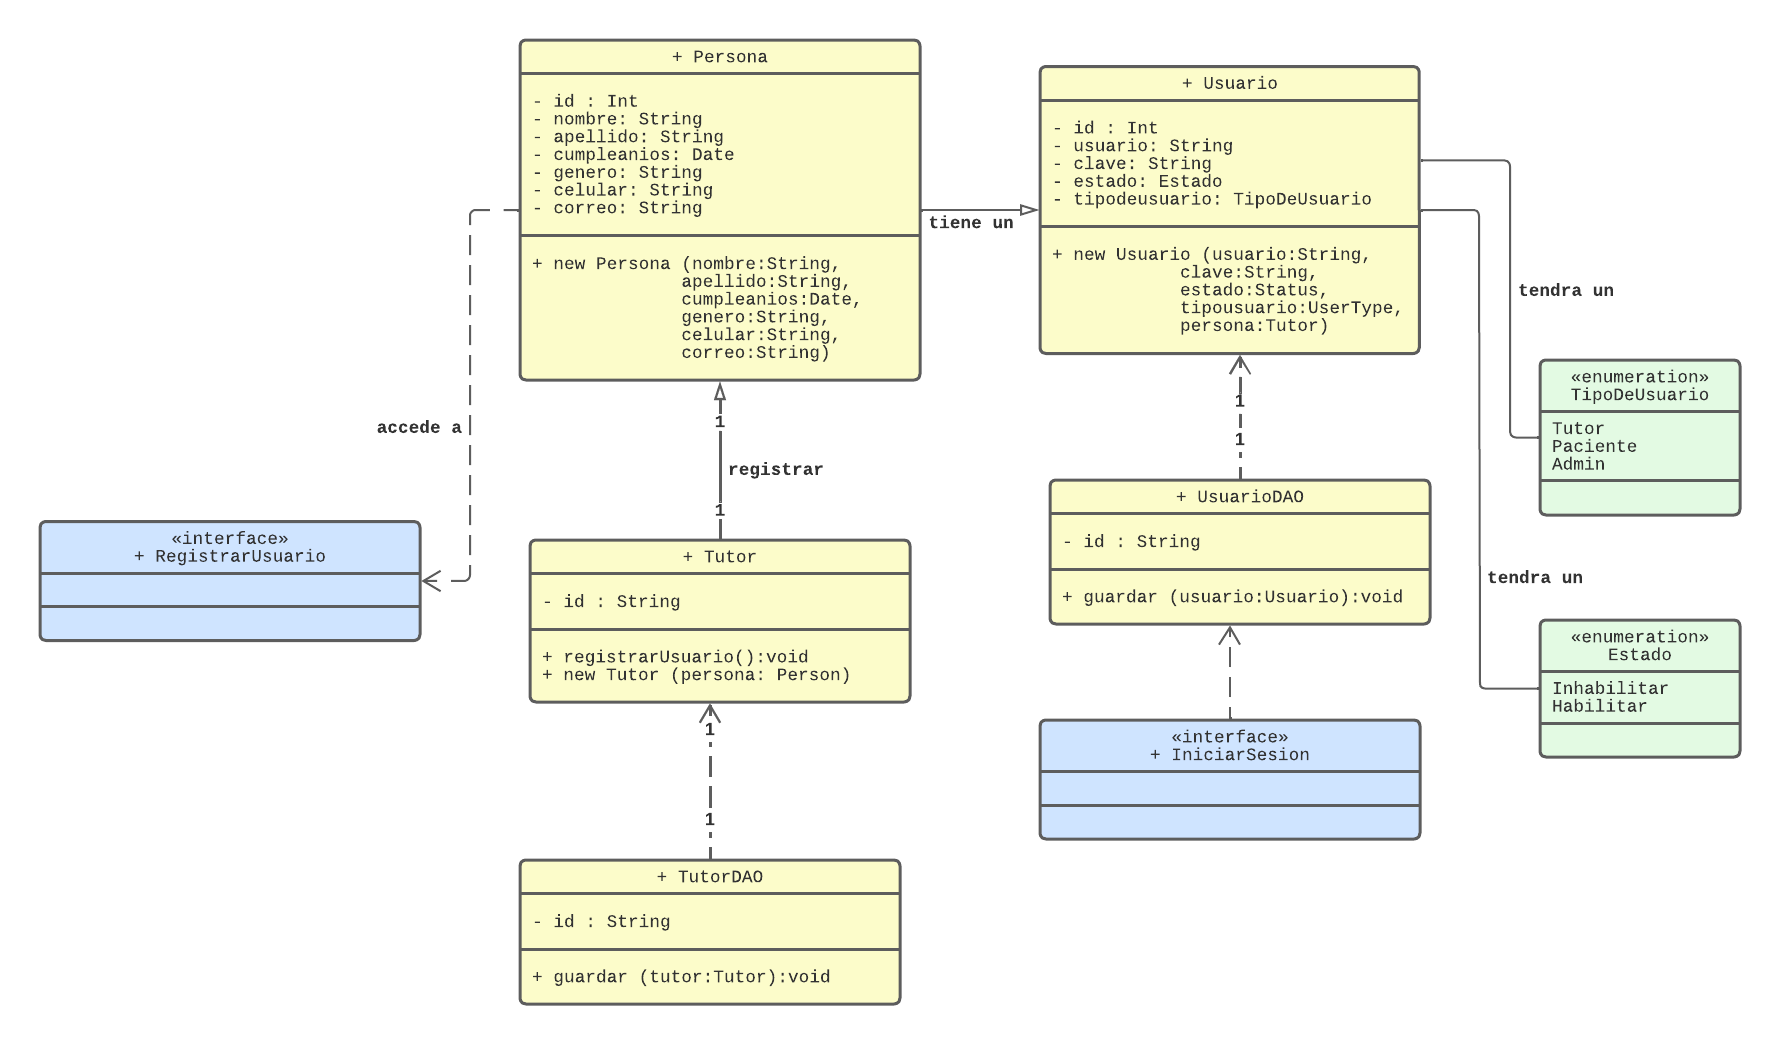
\includegraphics[width=13.2cm]{img/cdtest.png}
	\label{fig:cdtest}
	\vspace{4mm}
	{\footnotesize \textbf{\\ FUENTE: INVESTIGACIÓN} \textbf{\\ ELABORADO: AUTOR}}
\end{figure}

\begin{table}[h!]
	\caption{Descripción del caso de uso para registrar tutor.}
	\label{tab:usecasetutorregistration_symbol}
	\begin{tabular}{| p{3cm} | p{11cm} |}
		\hline
		\textbf{Caso de uso:} & Registrar de tutor \\ \hline
		\textbf{Actores:} & Persona \\ \hline
		\textbf{Poscondición:} & Usuario registrado en la base de datos. \\ \hline
		\textbf{Precondición:} & El usuario existe en la base de datos. \\ \hline
		\textbf{Propósito:} & Ingresar a la interfaz principal de la aplicación \\ \hline
		\textbf{Resumen:} & 
		Permite identificar las credenciales del usuario que intenta ingresar al sistema, de esa forma verificar el tipo de usuario que ingresa. \\ \hline
		\textbf{Tipo:} & Primario \\ \hline
		\multicolumn{2}{ |c| }{\textbf{Flujo normal}} \\ \hline
	\end{tabular}
	\begin{tabular}{| p{7cm} | p{7cm} |}
		1. Este caso de uso comienza cuando una *(/persona/ \&-id=int) quiere registrarse como usuario *(/tutor/ \&-id=int [+usuarioRegistrar=Tutor]) en el sistema. *¡tutor 1<[registro]>n Persona! & \\ \hline
		2. La persona accede entonces a la interfaz de *(@/Registro de Usuarios/). *¡Persona1<[accede]<1 Registro de Usuario! & \\ \hline

	\end{tabular}
\end{table}

\begin{table}[]
	\centering
	\begin{tabular}{| p{7cm} | p{7cm} |}
		\hline
		& 3. Muestra los campos a rellenar en la interfaz de *(@/Registro de usuarios/): *(Persona \&-/nombre/=String, \&-apellido/=String, \&-/fecha de nacimiento/=Date, \&-/género/=String, \&-/número de teléfono/=String, \&-/email/=String) *(Usuario \&-id=Int, \&-/nombreusuario/=String, \&-/clave/=String \&-estado=Status \&-tipo de usuario=UserType). Hay que tener en cuenta que el registro de una *!/Persona/ u<[/tiene un/]>u /Usuario/¡. Hay estados que pueden ser *¿Estado "/Deshabilitado/ /o/ "/Habilitado/? que cada *¡/Usuario/ u>[/tendrá un/]<u /Estado/! . También hay varios tipos de usuarios, que son *¿Tipo de usuario "/Tutor/ /o/ "/Paciente/ /o/ "/Admin/? y cada *¡/Usuario/ u>[/tendrá un/]<u /Tipo de usuario/! Además, el sistema asigna un identificador al almacenarlo.  \\ \hline
		4. La persona introduce todos los datos requeridos por la vista, y hace clic en enviar. & \\ \hline
		& 5. Crear un objeto *(/persona/ \%.nombre=String, .apellido=String, .fechacumpleanios=Date, .genero=String, .celular=String, .correo=String\%). \\ \hline
		& 6. Crear un objeto *(/tutor/ \%.person=Person\%) \\ \hline
		& 7. Crear un objeto *(/usuario/ \%.nombreusuario=String, .clave=String, .estado=Status, .tipodeusuario=UserType, .persona=Tutor\%) \\ \hline
		& 8. *(TutorDAO \&id=Int [/Guarda/=Tutor{.tutor=Tutor}])r el tutor en la base de datos *¡TutorDAO<[]< tutor!. \\ \hline
		& 9. *(UserDAO \&-id=Int [/Guarda/=User{.user=User}])r el usuario en la base de datos *¡UserDAO <[]< User!. \\ \hline
		& 10. Este caso de uso finaliza cuando el sistema muestra la interfaz de  *(@/Login/). *¡Login u<[]<u UserDAO! \\ \hline
	\end{tabular} \\
\vspace{4mm}
{\footnotesize \textbf{\\ FUENTE: INVESTIGACIÓN} \textbf{\\ ELABORADO: AUTOR}}
\end{table}

\subsection{Modelamiento}

Se utilizó el lenguaje de programación JavaScript con la intención de generar un paquete totalmente exportable a otros proyectos que requieran utilizar la librería para generar sus propios diagramas con otras librerías de dibujo. Para empezar con el diseño o modelamiento de la librería se especificó el proceso normal que deberá seguir la al momento de recibir como datos de entrada las descripciones de los casos de uso. En la ilustración \ref{fig:armadillocasodeuso} se observa el proceso que se llevará a cabo de forma general la ejecución de la librería.

En la ilustración \ref{fig:armadillocasodeuso} se puede observar el diagrama de casos de uso que explica las acciones que el analista podrá realizar al momento de implementar Armadillo.


\begin{figure}[h!]
	\centering
	\caption{Diagrama de casos de uso armadillo.}
	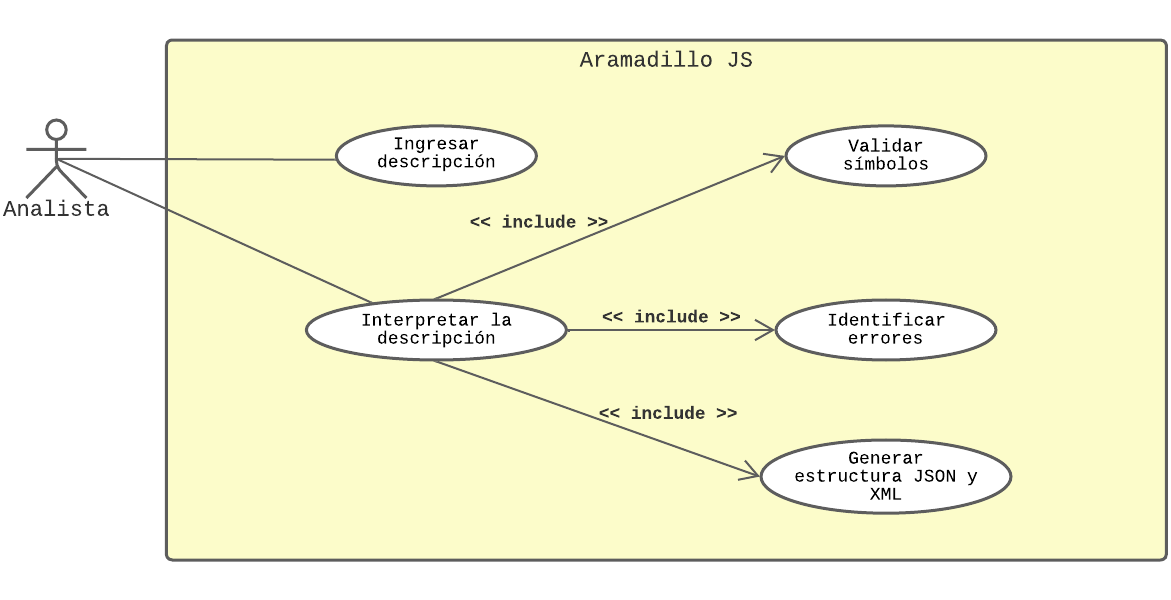
\includegraphics[width=15cm]{img/modelamientocasodeuso.png}
	\label{fig:armadillocasodeuso}
	\vspace{4mm}
	{\footnotesize \textbf{\\ FUENTE: INVESTIGACIÓN} \textbf{\\ ELABORADO: AUTOR}}
\end{figure} 

A continuación, se detallarán las descripciones de los casos de uso que se observan en la imagen anterior. Se especificarán todos los pasos que la librería debe recibir para responder de forma correcta. Se recuerda que Armadillo no cuenta con acceso a datos o algún tipo de información en la nube.  

\newpage

En la tabla \ref{tab:ucingresardescripcion} se detallan los pasos que se siguen al momento de ingresar las descripciones de los casos de uso que se pretenden interpretar.

\begin{table}[h!]
	\centering
	\caption{Descripción del caso de uso para interpretar la descripción.}
	\label{tab:ucinterpretardescripcion}
	\begin{tabular}{| p{3cm} | p{11cm} |}
		\hline
		\textbf{Caso de uso:} & Interpretar descripción \\ \hline
		\textbf{Actores:} & Analista \\ \hline
		\textbf{Precondición:} & Tener ingresada la descripción a interpretar redactada con el lenguaje de símbolos. \\ \hline
		\textbf{Postcondición:} & Obtener la descripción redactada en lenguaje natural. \\ \hline
		\textbf{Propósito:} & Obtener la descripción del caso de uso e interpretar los símbolos del lenguaje. \\ \hline
		\textbf{Resumen:} & Permite identificar cada símbolo del lenguaje para identificar los objetos que se deben crear en el diagrama de clases. \\ \hline
		\textbf{Tipo:} & Primario \\ \hline
		\multicolumn{2}{ |c| }{\textbf{Flujo normal}} \\ \hline
	\end{tabular}
	\begin{tabular}{| p{7cm} | p{7cm} |}
		\textbf{Acción del actor} & \textbf{Respuesta del sistema} \\ \hline	
		1. Este caso de uso inicia cuando el analista pretende interpretar la descripción del caso de uso. & \\ \hline		
		2. El analista da la orden de interpretar la descripción con el lenguaje de símbolos. & \\ \hline
		& 3. Muestra dentro de un apartado denominado consola, todos los procesos que realizaron al momento de interpretar la descripción. Además de mostrar rápidamente el texto redactado en lenguaje normal. \\ \hline
		4. El analista se dirige a la pestaña de "Class diagram".  & \\ \hline
		& 5. Muestra el grafico del diagrama de clases generado por la librería. Se dibujan los objetos que pudieron ser identificados por los símbolos usados. \\ \hline
		6. El analista se dirige a la pestaña de "JSON". & \\ \hline
		& 7. Muestra la estructura JSON generada. \\ \hline
		8. El analista se dirige a la pestaña de "XML".  & \\ \hline
		& 9. Muestra la estructura XML generada. \\ \hline
		10. Este caso de uso finaliza cuando el analista descarga las estructuras JSON o XML para posteriores proyectos. & \\ \hline			
	\end{tabular} \\
	\vspace{4mm}
	{\footnotesize \textbf{\\ FUENTE: INVESTIGACIÓN} \textbf{\\ ELABORADO: AUTOR}}
\end{table}


\begin{table}[h!]
	\centering
	\caption{Descripción del caso de uso para ingresar la descripción.}
	\label{tab:ucingresardescripcion}
	\begin{tabular}{| p{3cm} | p{11cm} |}
		\hline
		\textbf{Caso de uso:} & Ingresar descripción \\ \hline
		\textbf{Actores:} & Analista \\ \hline
		\textbf{Precondición:} & Tener instanciada la librería en su proyecto web, o debe utilizar la aplicación de demostración. \\ \hline
		\textbf{Postcondición:} & Descripción ingresada en la librería. \\ \hline
		\textbf{Propósito:} & Ingresar un párrafo de la descripción del caso de uso. \\ \hline
		\textbf{Resumen:} & Permite ingresar un párrafo de toda la descripción del caso de uso utilizando el lenguaje de símbolos. \\ \hline
		\textbf{Tipo:} & Primario \\ \hline
		\multicolumn{2}{ |c| }{\textbf{Flujo normal}} \\ \hline
	\end{tabular}
	\begin{tabular}{| p{7cm} | p{7cm} |}
		\centering
		\textbf{Acción del actor} & \textbf{Respuesta del sistema} \\ \hline	
		1. Este caso de uso inicia el analista ingresa la descripción del caso de uso. & \\ \hline
		& 2. Muestra la caja de texto donde se debe colocar la descripción del caso de uso con el lenguaje de símbolos. \\ \hline
		3. Este caso de uso finaliza cuando el analista ingresa la descripción del caso de uso. & \\ \hline
	\end{tabular}
	\vspace{4mm}
	{\footnotesize \textbf{\\ FUENTE: INVESTIGACIÓN} \textbf{\\ ELABORADO: AUTOR}}
\end{table}

\begin{table}[h!]
	\centering
	\caption{Descripción del caso de uso para generar estructura json y xml.}
	\label{tab:ucgenerarjsonxml}
	\begin{tabular}{| p{3cm} | p{11cm} |}
		\hline
		\textbf{Caso de uso:} & Generar estructura JSON y XML \\ \hline
		\textbf{Actores:} & Analista \\ \hline
		\textbf{Precondición:} & La descripción del caso de uso debe contar con SymLen. \\ \hline
		\textbf{Postcondición:} & Todos los símbolos serán omitidos en el texto interpretado. \\ \hline
		\textbf{Propósito:} & Generar 2 estructuras con la información del diagrama de clases. \\ \hline
		\textbf{Resumen:} & Permite obtener toda la estructura del diagrama de clases generado en formato JSON Y XML \\ \hline
		\textbf{Tipo:} & Secundario \\ \hline
		\multicolumn{2}{ |c| }{\textbf{Flujo normal}} \\ \hline
	\end{tabular}
	\begin{tabular}{| p{7cm} | p{7cm} |}
		\textbf{Acción del actor} & \textbf{Respuesta del sistema} \\ \hline	
		& 1. Este caso de uso inicia cuando la descripción del caso fue ingresada con los símbolos del lenguaje. \\ \hline
		& 2. Buscar los objetos que fueron identificados por los símbolos. \\ \hline
		& 3. Este caso de uso finaliza cuando se muestra el json y xml del diagrama de clases  \\ \hline		
	\end{tabular}
	\vspace{4mm}
	{\footnotesize \textbf{\\ FUENTE: INVESTIGACIÓN} \textbf{\\ ELABORADO: AUTOR}}
\end{table}

\begin{table}[h!]
	\centering
	\caption{Descripción del caso de uso para validar símbolos.}
	\label{tab:ucvalidarsimbolos}
	\begin{tabular}{| p{3cm} | p{11cm} |}
		\hline
		\textbf{Caso de uso:} & Validar símbolos \\ \hline
		\textbf{Actores:} & Analista \\ \hline
		\textbf{Precondición:} & La descripción del caso de uso debe contar con los símbolos del lenguaje. \\ \hline
		\textbf{Postcondición:} & Todos los símbolos serán omitidos en el texto que sea interpretado. \\ \hline
		\textbf{Propósito:} & Identificar los objetos para generar el diagrama de clases \\ \hline
		\textbf{Resumen:} & Permite identificar los símbolos que son usados para redactar los casos de uso. Además de verificar si se los esta usando de forma correcta. \\ \hline
		\textbf{Tipo:} & Secundario \\ \hline
		\multicolumn{2}{ |c| }{\textbf{Flujo normal}} \\ \hline
	\end{tabular}
	\begin{tabular}{| p{7cm} | p{7cm} |}
		\textbf{Acción del actor} & \textbf{Respuesta del sistema} \\ \hline	
		& 1. Este caso de uso inicia cuando la descripción del caso fue ingresada con los símbolos del lenguaje. \\ \hline
		& 2. Se identifican los tipos de símbolos que tiene el lenguaje, si son símbolos con apertura y cierre o son individuales. \\ \hline
		& 3. Se verifica que los símbolos están usándose de forma correcta sin combinarlos con otros símbolos desconocidos.  \\ \hline
		& 4. Este caso de uso finaliza cuando se identificaron todos los símbolos de la descripción y oculta los símbolos para obtener un texto natural.  \\ \hline		
	\end{tabular}
	\vspace{4mm}
	{\footnotesize \textbf{\\ FUENTE: INVESTIGACIÓN} \textbf{\\ ELABORADO: AUTOR}}
\end{table}

\begin{table}[h!]
	\centering
	\caption{Descripción del caso de uso para identificar errores.}
	\label{tab:ucidentificarerror}
	\begin{tabular}{| p{3cm} | p{11cm} |}
		\hline
		\textbf{Caso de uso:} & Identificar errores \\ \hline
		\textbf{Actores:} & Analista \\ \hline
		\textbf{Precondición:} & La descripción del caso de uso debe contar con los símbolos del lenguaje. \\ \hline
		\textbf{Postcondición:} & Todos los símbolos serán omitidos en el texto que sea interpretado. \\ \hline
		\textbf{Propósito:} & Permite identificar la mala escritura de las descripciones de los casos de uso. \\ \hline
		\textbf{Resumen:} & Identificar los posibles errores que se pueden cometer al momento de usar los símbolos en las descripciones de los casos de uso. \\ \hline
		\textbf{Tipo:} & Secundario \\ \hline
	\end{tabular}
\end{table}

\begin{table}
	\centering
	\begin{tabular}{| p{7cm} | p{7cm} |}
		\hline
		\multicolumn{2}{ |c| }{\textbf{Flujo normal}} \\ \hline
		\textbf{Acción del actor} & \textbf{Respuesta del sistema} \\ \hline	
		& 1. Este caso de uso inicia cuando la descripción del caso fue ingresada con los símbolos del lenguaje. \\ \hline
		& 2. Se identifican los tipos de símbolos que tiene el lenguaje, si son símbolos con apertura y cierre o son individuales. \\ \hline
		& 3. Si existen inconsistencias en la redacción de la descripción del caso de uso, se empieza acumular mensajes de alerta.   \\ \hline
		& 4.  Este caso de uso finaliza mostrando los mensajes en un apartado y clasificando los mensajes acumulados mediante un color diferentes: Azul para información, amarillo para advertencia, verde para exitoso y rojo para notificar errores graves. \\ \hline		
	\end{tabular}
	\vspace{4mm}
	{\footnotesize \textbf{\\ FUENTE: INVESTIGACIÓN} \textbf{\\ ELABORADO: AUTOR}}
\end{table}

%Para cumplir con los requisitos recopilados en la fase anterior se realizaron diagramas de flujo para realizar el análisis pertinente a lo que la librería debe cumplir. Esto permitirá identificar las posibles fallas que se mostrarían al momento de estar utilizando la librería. En la ilustración \ref{fig:algoritmoerror} se observa el algoritmo que permitió identificar los errores en la escritura de las descripciones de los casos de uso utilizando el lenguaje de símbolos.

%\lstinputlisting[language=JavaScript]{codigo/pseudocodigo.txt}

%\begin{figure}[h!]
%	\centering
%	\caption{Diagrama de flujo para detectar errores en las descripciones de los casos de uso utilizando SymLen.}
%	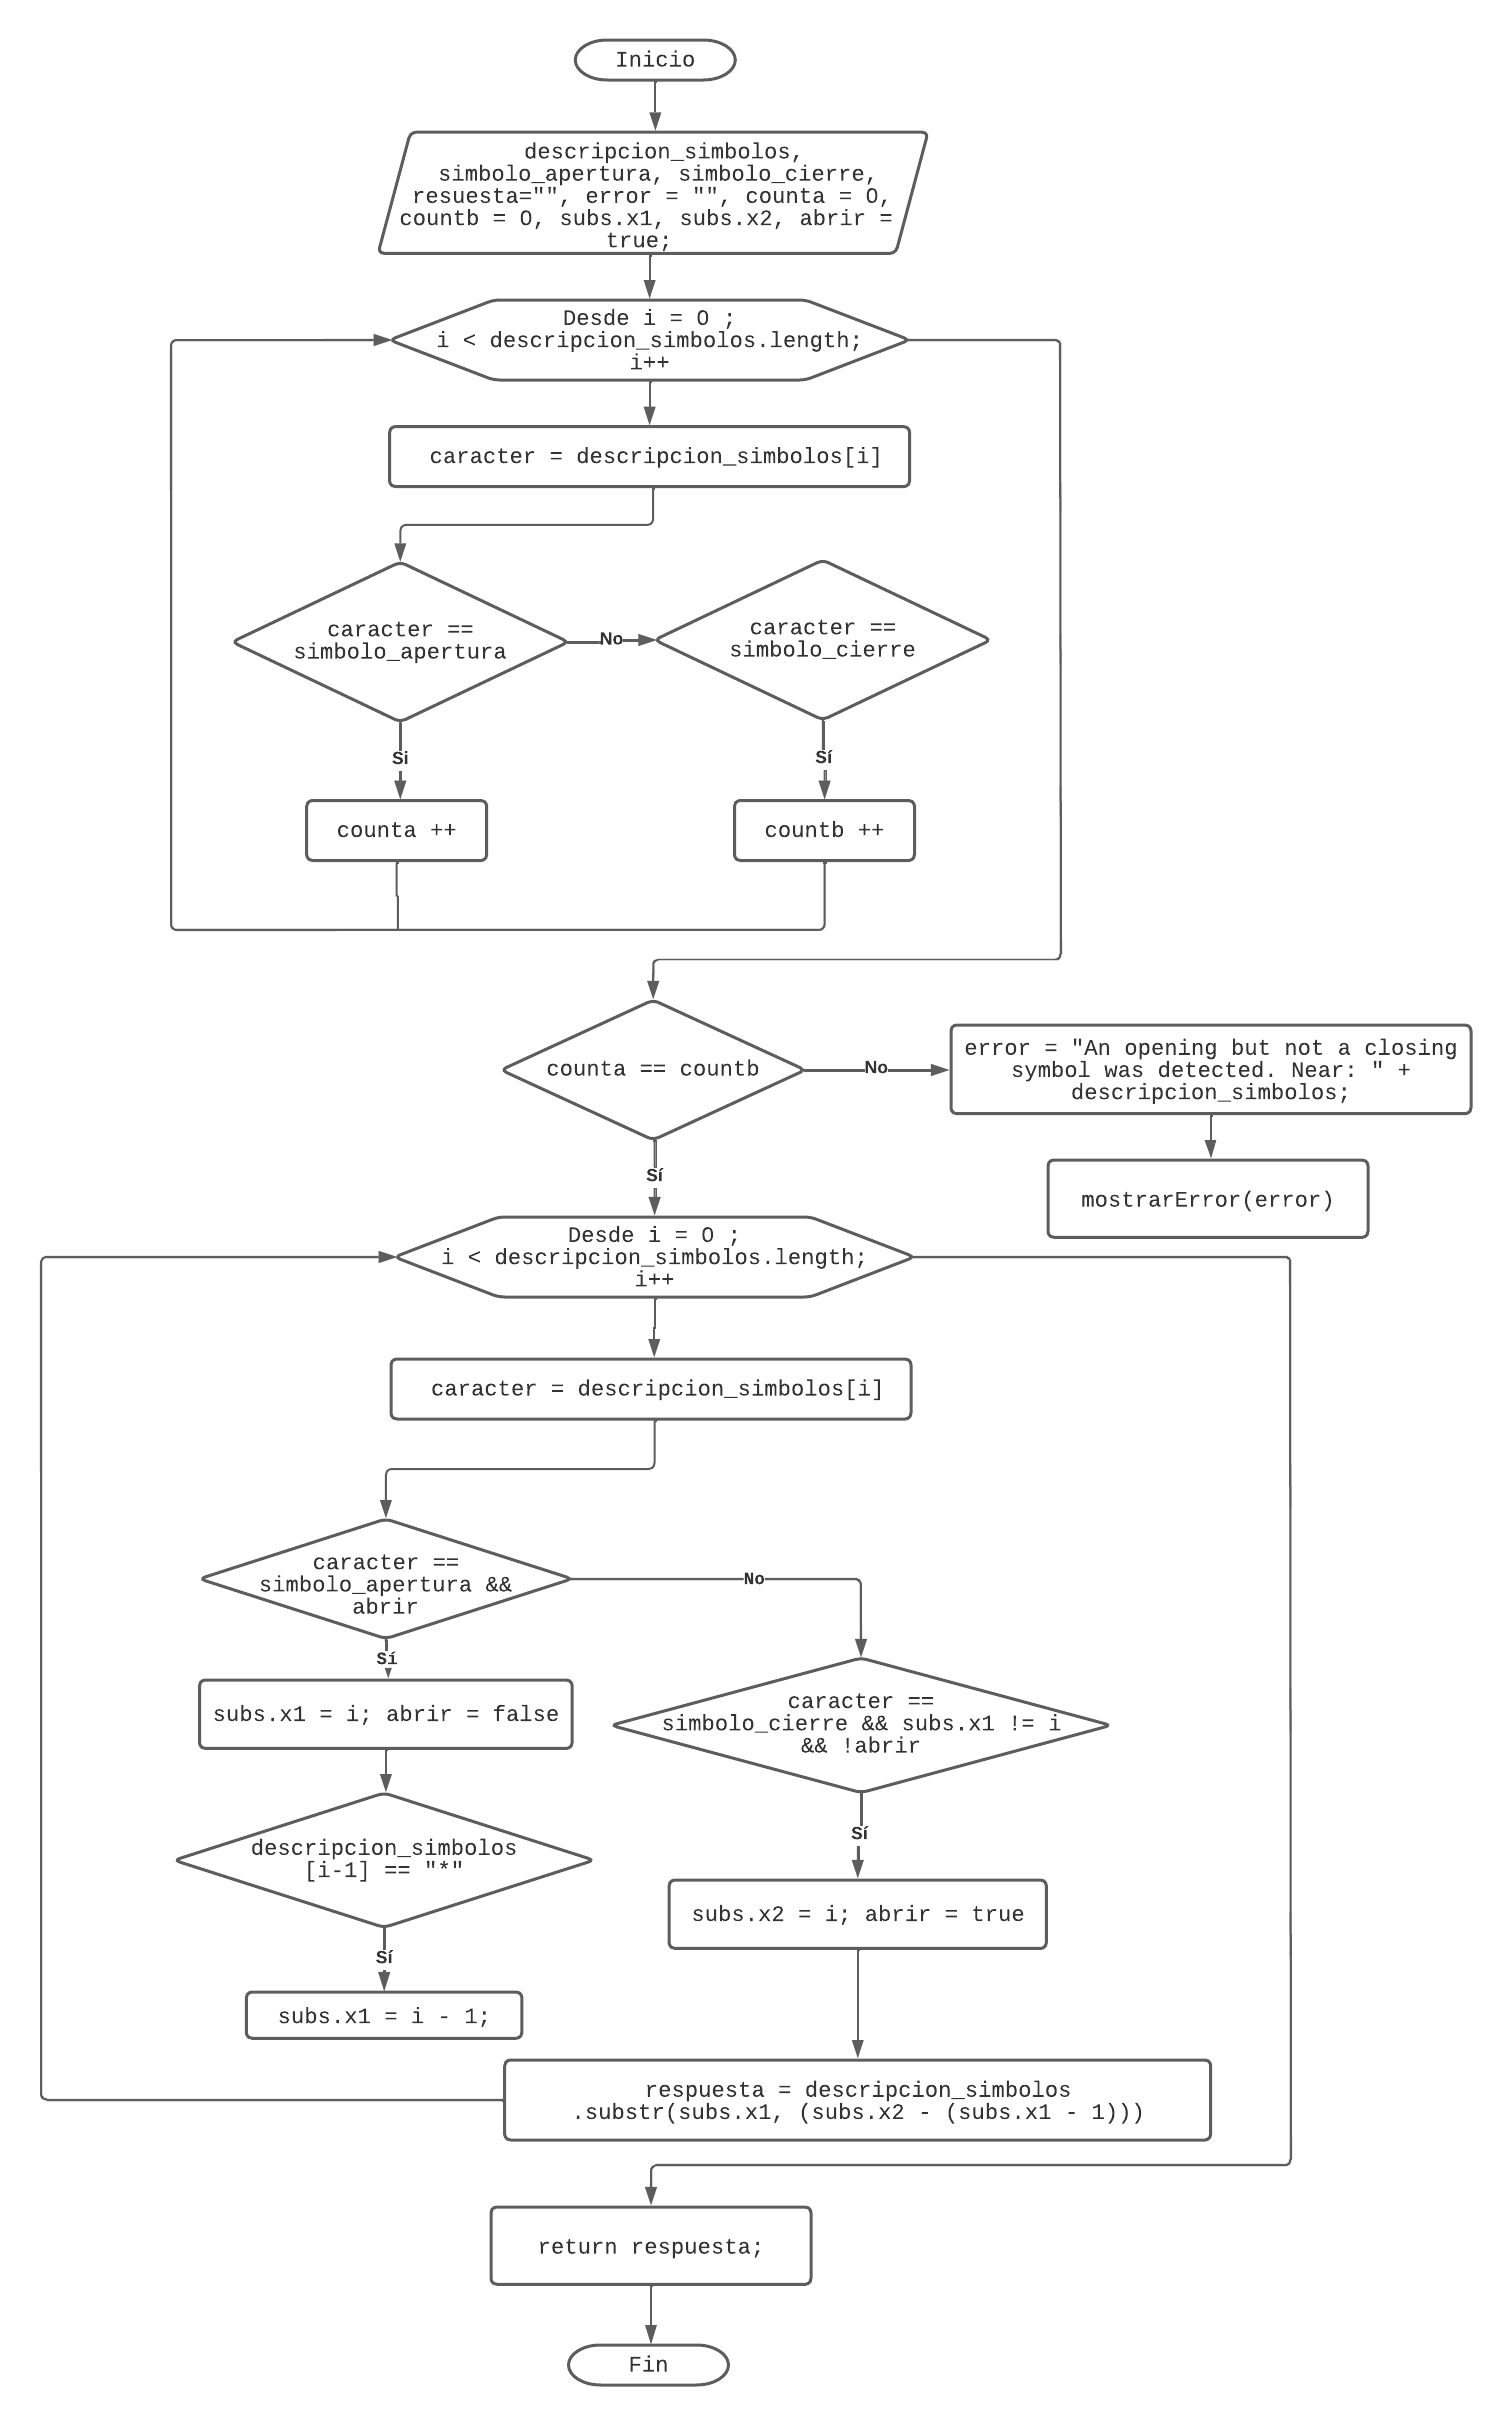
\includegraphics[width=13cm]{img/algoritmoerror.png}
%	\label{fig:algoritmoerror}
%	\vspace{4mm}
%	{\footnotesize \textbf{\\ FUENTE: INVESTIGACIÓN} \textbf{\\ ELABORADO: %AUTOR}}
%\end{figure} 

%\newpage

\subsection{Generación de código}

En la siguiente fase se desarrollaron las funciones y todos los métodos que fueron necesarios para que la librería funcione correctamente. A continuación, se observan todas las variables que fueron necesarias para que todo funcione de manera correcta.

\lstinputlisting[language=JavaScript]{codigo/variables.js}

En el siguiente bloque de código se observa la función que permite acumular los mensajes de error que pueden ocurrir al momento de interpretar las descripciones de los casos de uso. 

\lstinputlisting[language=JavaScript]{codigo/notificaciones.js}

En el siguiente bloque de código se observa una de las funciones principales para detectar los símbolos de apertura y cierre, con el objetivo de utilizar una sola función que permita identificar los símbolos que necesariamente deben ser con apertura y cierre. 

\lstinputlisting[language=JavaScript]{codigo/detectarsimbolos.js}

Para mejorar la presentación de la librería se desarrolló una aplicación web sencilla que permita utilizar de forma gráfica las funciones de esta. La aplicación web tendrá como propósito proporcionar un lugar en la web de donde descargar el script para que pueda ser usado por la comunidad de desarrolladores. Además, de proporcionar documentación de como instalarla en otros proyectos y como utilizarla. 

\subsection{Ejecución de pruebas}

Para la ejecución de las pruebas, se analizó el caso de uso que fue proporcionado por el docente. Cada párrafo estaba redactado con el lenguaje de símbolos, por lo que se ingresaron las descripciones en la aplicación de demostración y los resultados fueron los siguientes:

\sloppy
\begin{itemize}
	\item Descripción \#1:
	\begin{lstlisting} 
		Este caso de uso comienza cuando una *(/persona/ &-id=int) quiere registrarse como usuario *(/tutor/ &- id=int [+usuarioRegistrar=Tutor]) en el sistema. *¡tutor 1<[registro]>n Persona! \end{lstlisting}

	Interpretando el párrafo, se creó una clase denominada Tutor con sus respectivos atributos que son: \textbf{id} privado y de tipo String, los métodos que se agregaron son: \textbf{usuarioRegistrar()} público. Además, se realizó una relación de tipo generalización. A continuación, se observa la estructura json y xml generada por la librería a partir del párrafo ingresado.

\lstinputlisting[language=JavaScript]{codigo/pruebas/test01.json}
\lstinputlisting[language=JavaScript]{codigo/pruebas/test01.xml}

Para que la descripción del caso de uso pueda ser entendida por el cliente del sistema que se esté desarrollando se obtiene como resultado el párrafo redactado en lenguaje natural omitiendo los símbolos y pueda ser comprendido con mayor facilidad.

	\begin{lstlisting}
		Este caso de uso comienza cuando una persona quiere registrarse como usuario tutor en el sistema.  \end{lstlisting}
	
	Como el texto está redactado de forma correcta la retroalimentación generada muestra mensajes exitosos:
	
	\textcolor{blue}{\textbf{información:} Descripción ingresada: Este caso de uso comienza cuando una *(/persona/ \&-id=int) quiere registrarse como usuario *(/tutor/ \&- id=int [+usuarioRegistrar=Tutor]) en el sistema. *¡tutor 1<[registro]>n Persona!}
	
	\textcolor{ForestGreen}{
		\textbf{éxito:} Atributos añadidos con éxito: id \\
		\textbf{éxito:} La clase Persona se ha generado con éxito \\
		\textbf{éxito:} Atributos añadidos con éxito: id \\
		\textbf{éxito:} La clase Tutor se ha generado con éxito \\
		\textbf{éxito:} La relación de generalización entre los objetos de: Tutor 1<>n to: Persona se ha generado con éxito. }
	
	Para verificar el funcionamiento de la retroalimentación identificando la mala escritura de las descripciones del caso de uso usando el lenguaje de símbolos, se redactó a propósito el mismo párrafo usando de forma incorrecta los símbolos.
	
	\begin{lstlisting}
		Este caso de uso comienza cuando una *(/persona/ &-id=int) quiere registrarse como usuario *(/tutor/ &- id=int [+usuarioRegistrar=Tutor]) en el sistema. *¡tutor 1<[registro]>n Persona \end{lstlisting} 
	
	Observando los menajes de retroalimentación ya se identificaron que errores se están cometiendo en el uso de algunos símbolos y especificando en qué lugar del texto se encuentra ese error.
	
	\textcolor{blue}{\textbf{información:} Descripción ingresada: Este caso de uso comienza cuando una *(/persona/ \&-id=int) quiere registrarse como usuario *(/tutor/ \&- id=int [+usuarioRegistrar=Tutor]) en el sistema. *¡tutor 1<[registro]>n Persona}
	
	\textcolor{ForestGreen}{
	\textbf{éxito:} Atributos añadidos con éxito: id \\
	\textbf{éxito:} La clase Persona se ha generado con éxito \\
	\textbf{éxito:} Atributos añadidos con éxito: id}

	\textcolor{Red}{
	\textbf{error:} Se ha detectado un símbolo de apertura pero no de cierre. => inicio: [, fin: ]. Cerca de: *(/tutor/ \&- id=int [+usuarioRegistrar=Tutor)}

	\textcolor{ForestGreen}{\textbf{éxito:} La clase Tutor se ha generado con éxito }
	
	\textcolor{Red}{
	\textbf{error:}  Se ha detectado un símbolo de apertura pero no de cierre. => begin: ¡, fin: !. Cerca: Este caso de uso comienza cuando una persona *(persona \&-id=int) quiere registrarse como usuario tutor *(tutor \&-id=int [+userRegistration=Tutor) en el sistema. *¡tutor 1<[registro]>n Persona}

	Utilizando la aplicación web de demostración, se logra observar ene la ilustración \ref{fig:prueba01} el diagrama de clases creado a partir de la estructura json o xml que la librería proporciona de forma automática. Para dibujar el diagrama de clases, se está utilizando la librería JavaScript jsUml2. 
	
	\begin{figure}[h!]
		\centering
		\caption{Diagrama de clases generado por la aplicación web de demostración usando la librería de armadillo.js, descripción 1}
		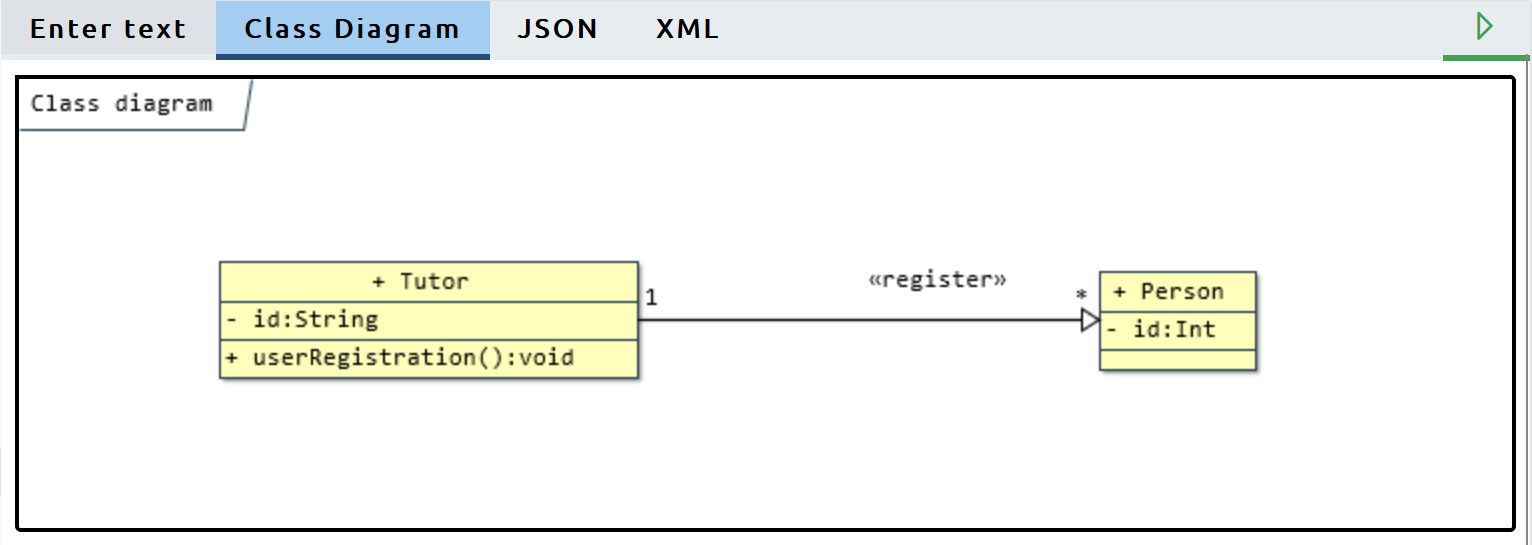
\includegraphics[width=15cm]{img/prueba01.png}
		\label{fig:prueba01}
		\vspace{4mm}
		{\footnotesize \textbf{\\ FUENTE: INVESTIGACIÓN} \textbf{\\ ELABORADO: AUTOR}}
	\end{figure}

	\sloppy
	\item \textbf{Descripción \#2:}
	\begin{lstlisting}
		La persona accede entonces a la interfaz de Registro de usuarios *(@Registro de Usuarios). *¡Persona1<[accede]<1 Registro de Usuarios! \end{lstlisting}

	A continuación, se evidenciará como se va modificando el diagrama de clases por cada descripción del caso de uso que se va interpretando hasta llegar al diagrama de clases final. En esta descripción se generó un nuevo objeto para el diagrama que es una interfaz denominada Registro de usuarios que se relaciona mediante dependencia a la clase Persona (ver ilustración \ref{fig:prueba02}).
	
	\begin{lstlisting}
		La persona accede entonces a la interfaz de Registro de usuarios \end{lstlisting} 
	
	\begin{figure}[h!]
		\centering
		\caption{Diagrama de clases generado por la aplicación web de demostración usando la librería de armadillo.js, descripción 2}
		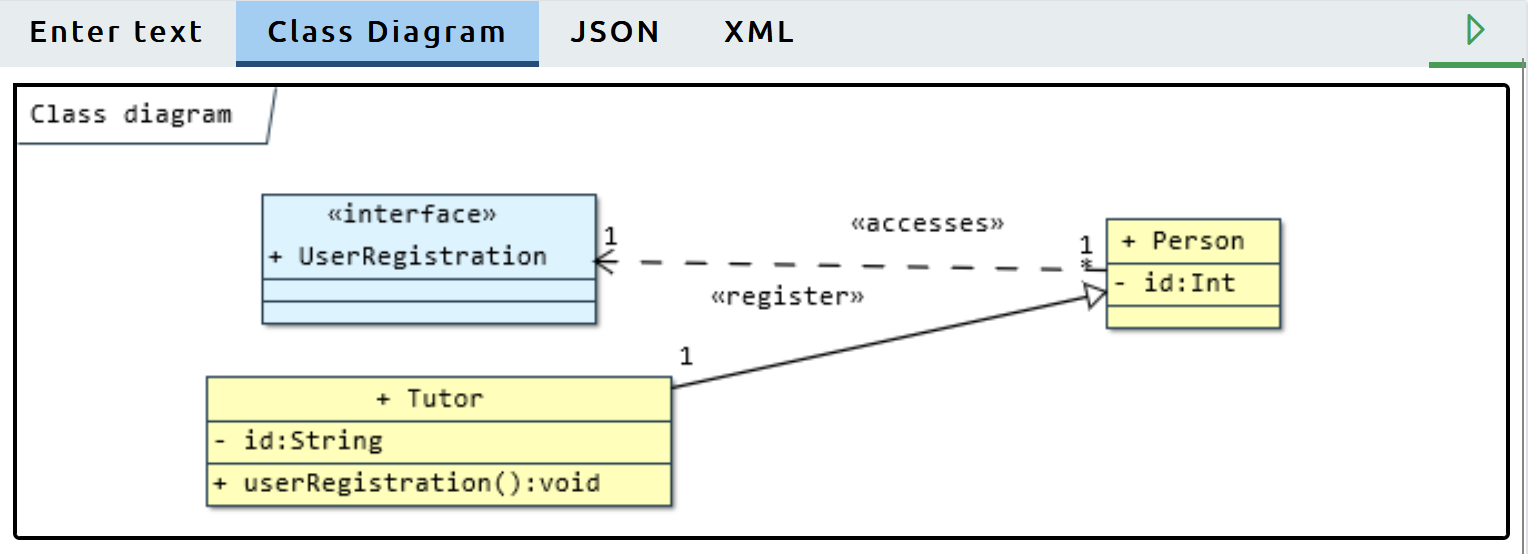
\includegraphics[width=15cm]{img/prueba02.png}
		\label{fig:prueba02}
		\vspace{4mm}
		{\footnotesize \textbf{\\ FUENTE: INVESTIGACIÓN} \textbf{\\ ELABORADO: AUTOR}}
	\end{figure}

	\item \textbf{Descripción \#3:}
	\begin{lstlisting}
		Muestra los campos a rellenar en la interfaz de *(@/Registro de usuarios/): *(Persona &-/nombre/=String, &- apellido/=String, &-/fecha de nacimiento/=Date, &-/género/=String, &-/número de teléfono/=String, &-/email/=String) *(Usuario &- id=Int, &-/nombreusuario/=String, &-/clave/=String &-estado=Status &- tipo de usuario=UserType). Hay que tener en cuenta que el registro de una *¡/Persona/ u<[/tiene un/]>u /Usuario/!. Hay estados que pueden ser *¿Estado"/Deshabilitado/ /o/ "/Habilitado/? que cada *¡/Usuario/ u>[/tendrá un/]<u /Estado/! . También hay varios tipos de usuarios, que son *¿Tipo de usuario"/Tutor/ /o/ "/Paciente/ /o/ "/Admin/? y cada *¡/Usuario/ u>[/tendrá un/]<u /Tipo de usuario/! Además, el sistema asigna un identificador al almacenarlo. \end{lstlisting}
	
		En esta descripción se detallaron más objetos del diagrama de clases. Se observa que se agregaron más atributos a la clase Persona, se agregaron 2 objetos enum que se denominan Estado y Tipo de usuario, aparte que están relacionados con la clase Usuario que también fue agregada en esta descripción.
		
		\begin{lstlisting}
		Muestra los campos a rellenar en la interfaz de Registro de usuarios: nombre nombreusuario clave. Hay que tener en cuenta que el registro de una Persona tiene un Usuario. Hay estados que pueden ser Deshabilitado o Habilitado que cada Usuario tendrá un Estado . También hay varios tipos de usuarios, que son Tutor o Paciente o Admin y cada Usuario tendrá un Tipo de usuario Además, el sistema asigna un identificador al almacenarlo. \end{lstlisting}

	\begin{figure}[h!]
		\centering
		\caption{Diagrama de clases generado por la aplicación web de demostración usando la librería de armadillo.js, descripción 3}
		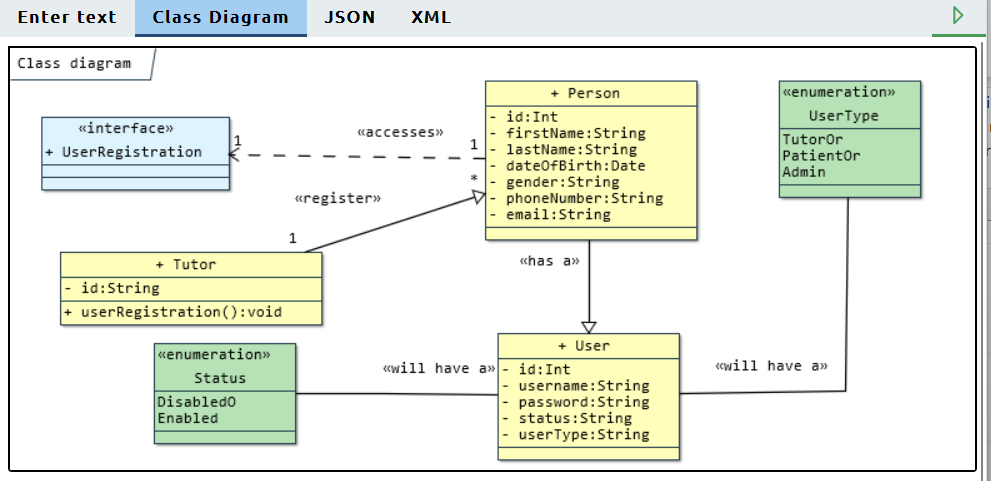
\includegraphics[width=15cm]{img/prueba03.png}
		\label{fig:prueba03}
		\vspace{4mm}
		{\footnotesize \textbf{\\ FUENTE: INVESTIGACIÓN} \textbf{\\ ELABORADO: AUTOR}}
	\end{figure}

	\item \textbf{Descripción \#4:}
	
	\begin{lstlisting}
		 Crear un objeto *(/persona/ %.nombre=String, .apellido=String, .fechacumpleanios=Date, .genero=String, .celular=String, .correo=String%). \end{lstlisting}
	
	En esta descripción se agregó un nuevo constructor para la clase Persona con los siguientes parámetros: nombre, apellido, fechacumpleanios, genero, numero de celular y correo.
	
	\begin{lstlisting}
		Crear un objeto persona.  \end{lstlisting}
	
	\begin{figure}[h!]
		\centering
		\caption{Diagrama de clases generado por la aplicación web de demostración usando la librería de armadillo.js, descripción 4}
		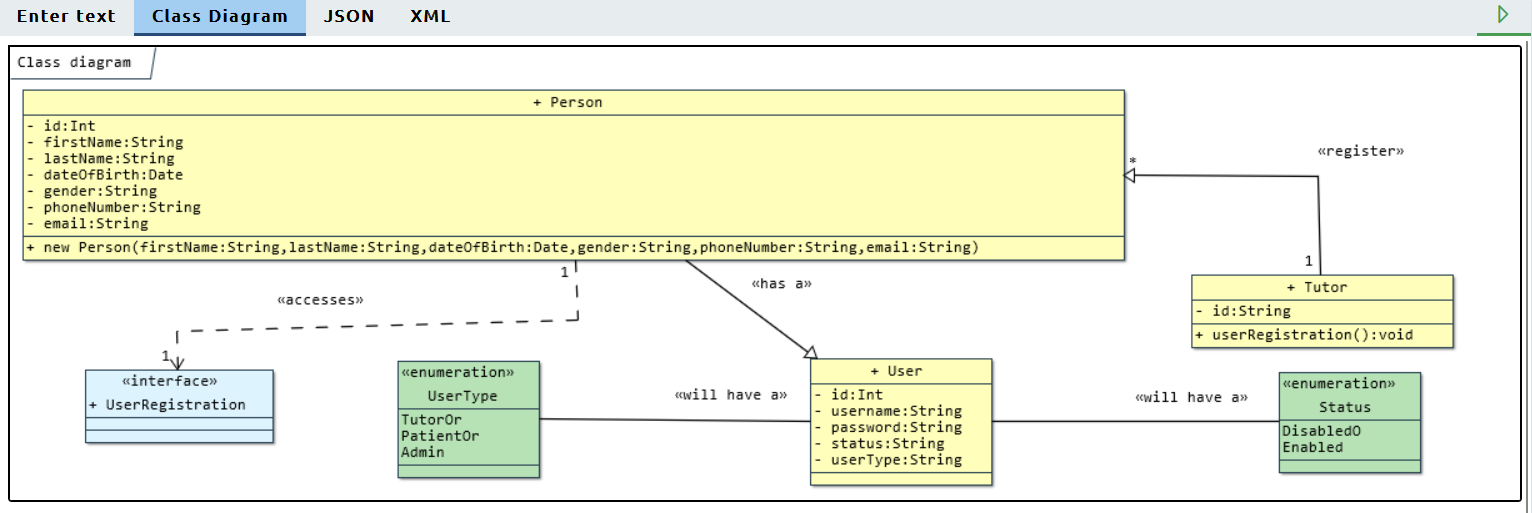
\includegraphics[width=15cm]{img/prueba04.png}
		\label{fig:prueba04}
		\vspace{4mm}
		{\footnotesize \textbf{\\ FUENTE: INVESTIGACIÓN} \textbf{\\ ELABORADO: AUTOR}}
	\end{figure}

	\item \textbf{Descripción \#5:}
	\begin{lstlisting}
		Crear un objeto *(/tutor/%.person=Person%) \end{lstlisting}

	En la siguiente descripción se agregó un nuevo constructor a la clase Tutor que recibe como parámetro un objeto de la clase Person. 
	
	\begin{lstlisting}
		Crear un objeto tutor  \end{lstlisting}
	
	\begin{figure}[h!]
		\centering
		\caption{Diagrama de clases generado por la aplicación web de demostración usando la librería de armadillo.js, descripción 5}
		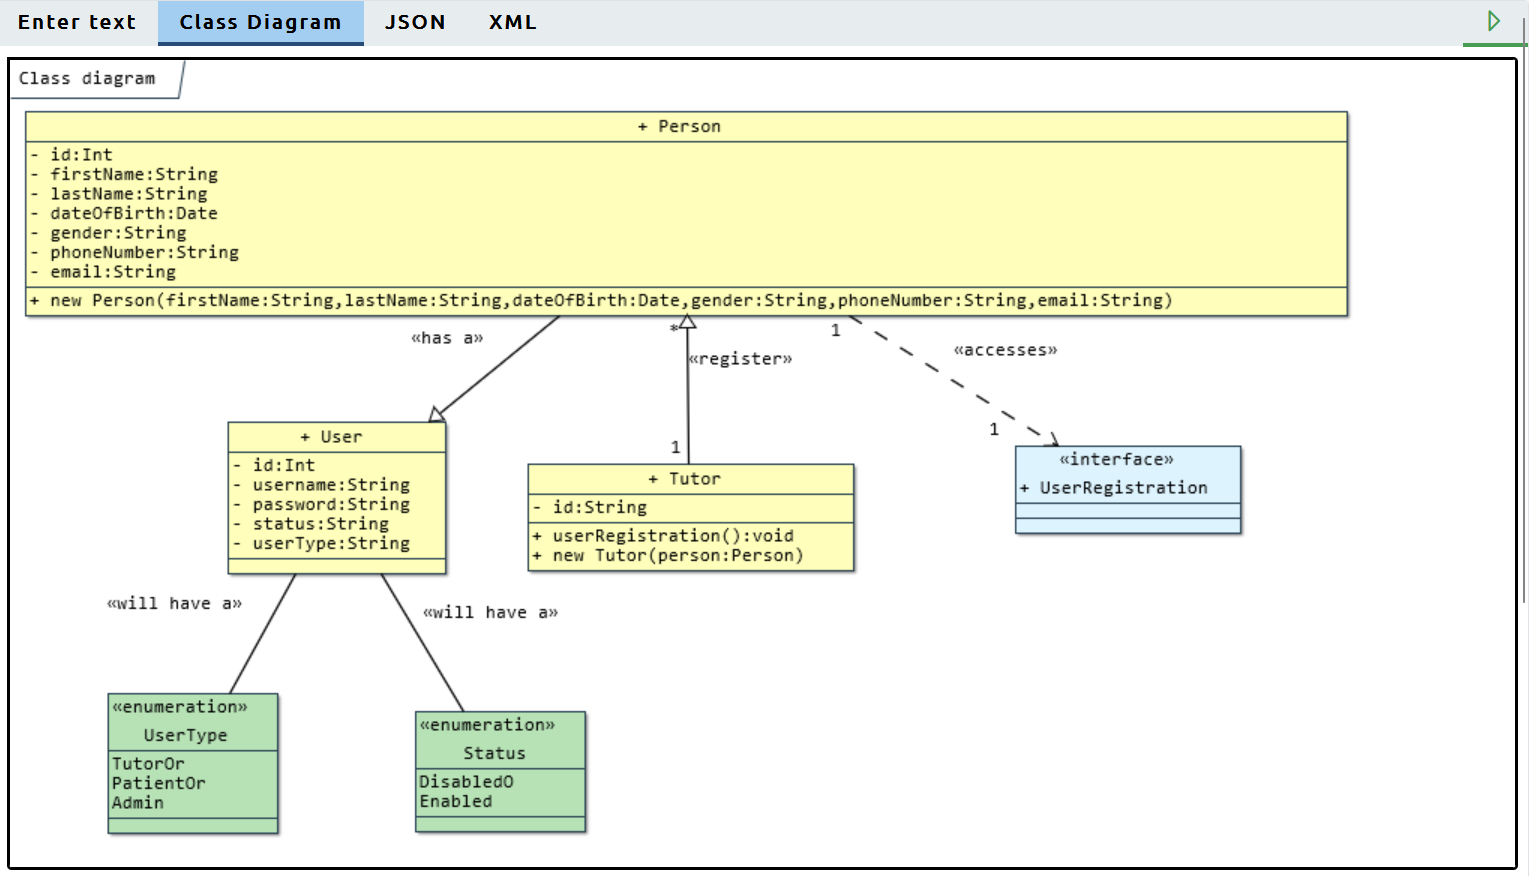
\includegraphics[width=15cm]{img/prueba05.png}
		\label{fig:prueba05}
		\vspace{4mm}
		{\footnotesize \textbf{\\ FUENTE: INVESTIGACIÓN} \textbf{\\ ELABORADO: AUTOR}}
	\end{figure}

	\item \textbf{Descripción \#6}
	\begin{lstlisting}
		 Crear un objeto *(/usuario/%.nombreusuario=String, .clave=String, .estado=Status, .tipodeusuario=UserType, .persona=Tutor%) \end{lstlisting}
	
	En la descripción se observa que se agregó un nuevo constructor a la clase User con sus parámetros que son: nombreusuario, clave, estado, tipodeusuario y persona que es un objeto Tutor. 
	
	\begin{lstlisting}
		Crear un objeto usuario  \end{lstlisting}
	
	\begin{figure}[h!]
		\centering
		\caption{Diagrama de clases generado por la aplicación web de demostración usando la librería de armadillo.js, descripción 6}
		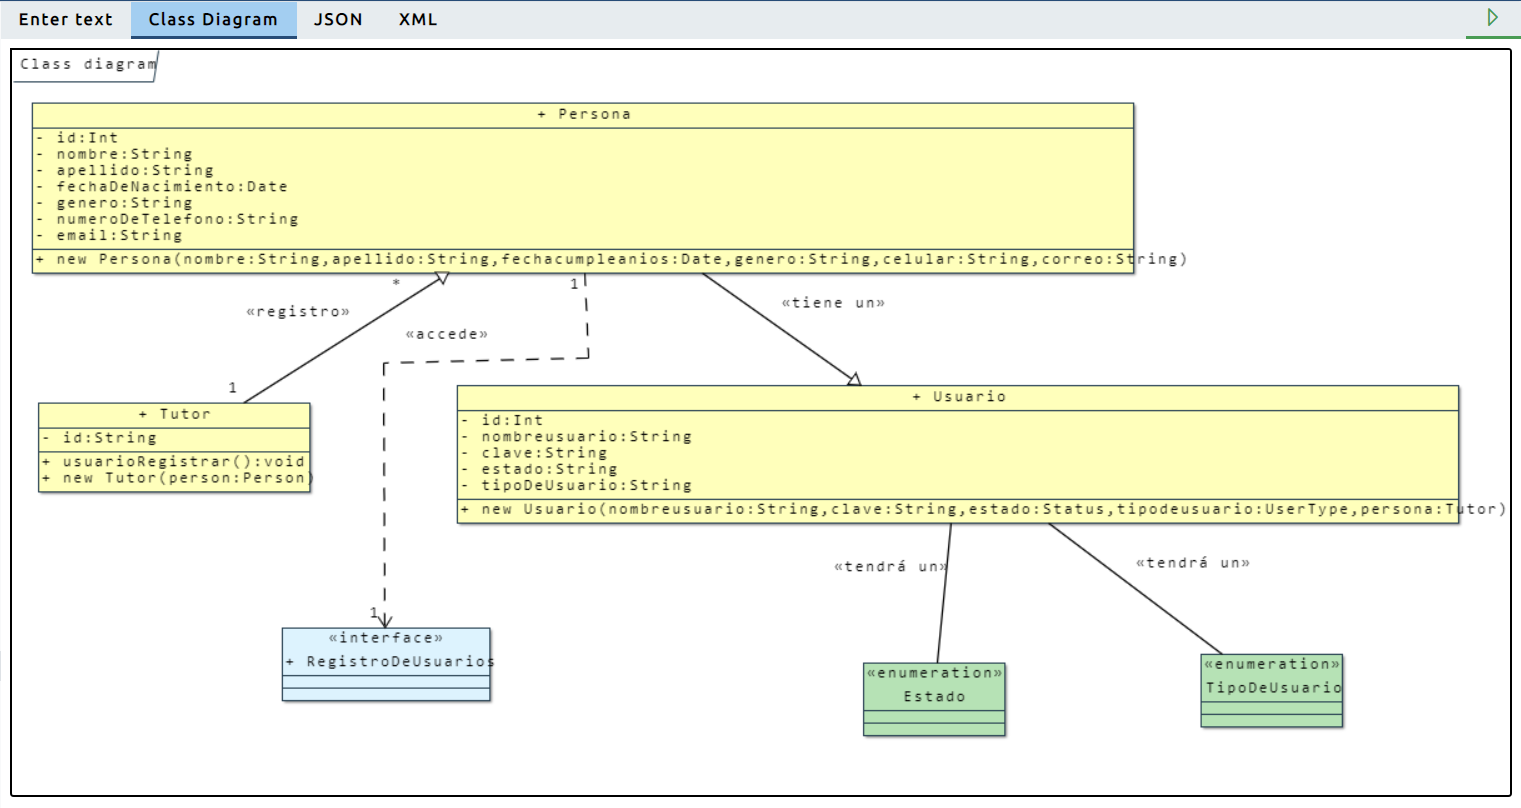
\includegraphics[width=15cm]{img/prueba06.png}
		\label{fig:prueba06}
		\vspace{4mm}
		{\footnotesize \textbf{\\ FUENTE: INVESTIGACIÓN} \textbf{\\ ELABORADO: AUTOR}}
	\end{figure}

	\item \textbf{Descripción \#7:}
	\begin{lstlisting}
		*(TutorDAO &id=Int [/Guarda/=Tutor.tutor=Tutor])r el tutor en la base de datos *¡TutorDAO<[]< tutor!. \end{lstlisting}
	
	En la siguiente descripción se observa que se agregó una nueva clase que se denomina TutorDAO. Se agregó un método que se llama Guardar que recibe como parámetro un objeto de tipo Tutor y retorna un objeto Tutor mismo. Además, se generó una relación de tipo Dependencia con la clase Tutor pero sin cardinalidad.
	\begin{lstlisting}
		Guardar el tutor en la base de datos. \end{lstlisting}
	
	\begin{figure}[h!]
		\centering
		\caption{Diagrama de clases generado por la aplicación web de demostración usando Armadillo, descripción 7}
		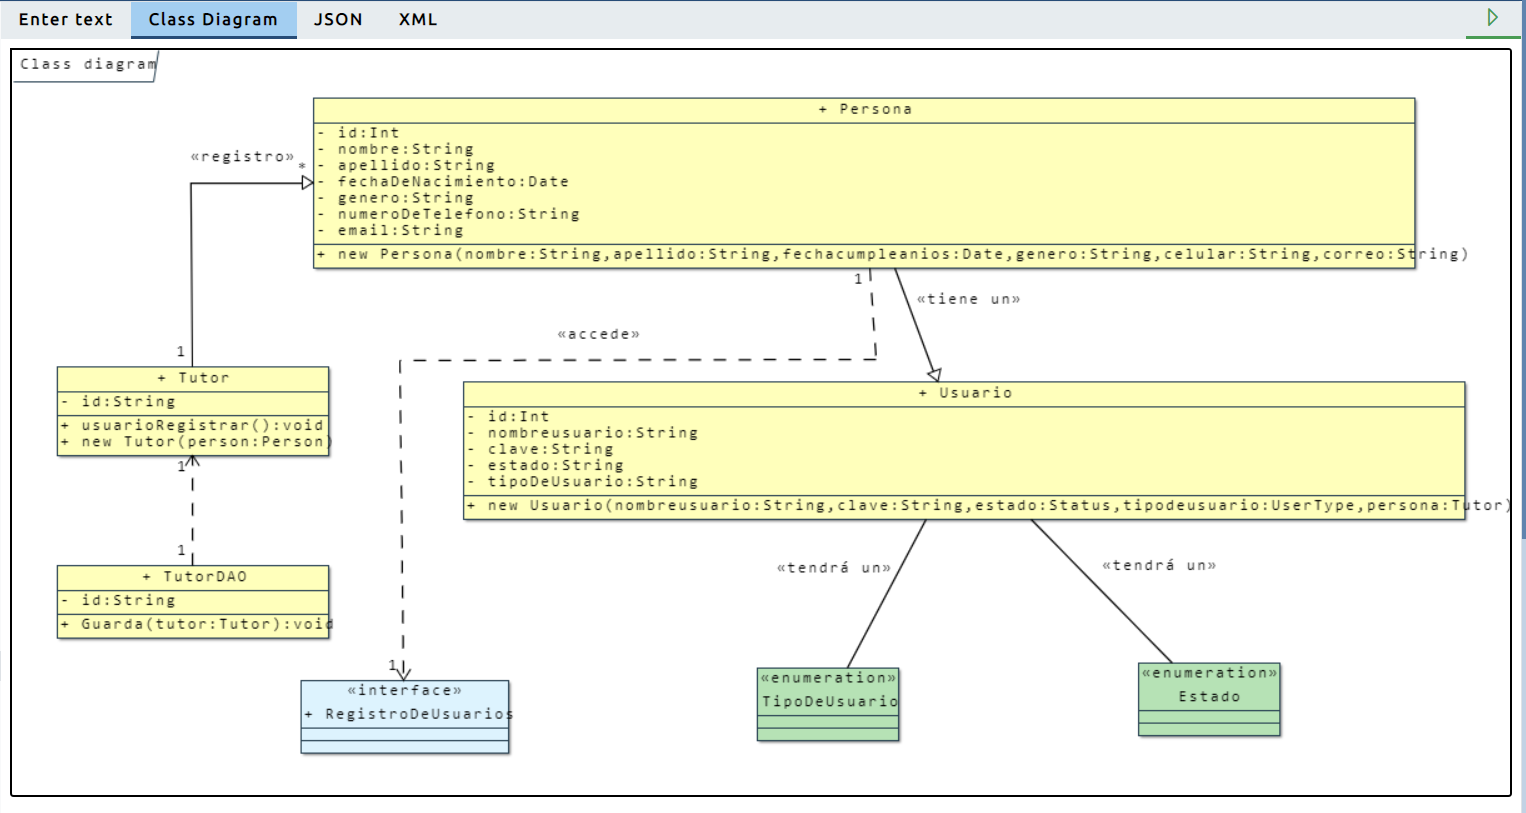
\includegraphics[width=15cm]{img/prueba07.png}
		\label{fig:prueba07}
		\vspace{4mm}
		{\footnotesize \textbf{\\ FUENTE: INVESTIGACIÓN} \textbf{\\ ELABORADO: AUTOR}}
	\end{figure}
	
	\item \textbf{Descripción \#8:}
	\begin{lstlisting}
	*(UserDAO &-id=Int [/Guarda/=User.user=User])r el usuario en la base de datos *¡UserDAO <[]< Usuario! \end{lstlisting}

	En la siguiente descripción se agregó una clase denominada UserDAO con un método llamado save que recibe como parámetro un objeto de tipo Usuario. Además, se relaciona mediante la relación de tipo Dependencia con la clase Usuario (ver ilustración \ref{fig:prueba08}).	
	
	\begin{lstlisting}
		Guardar el usuario en la base de datos \end{lstlisting}

	\begin{figure}[h!]
		\centering
		\caption{Diagrama de clases generado por la aplicación web de demostración usando la librería de armadillo.js, descripción 8}
		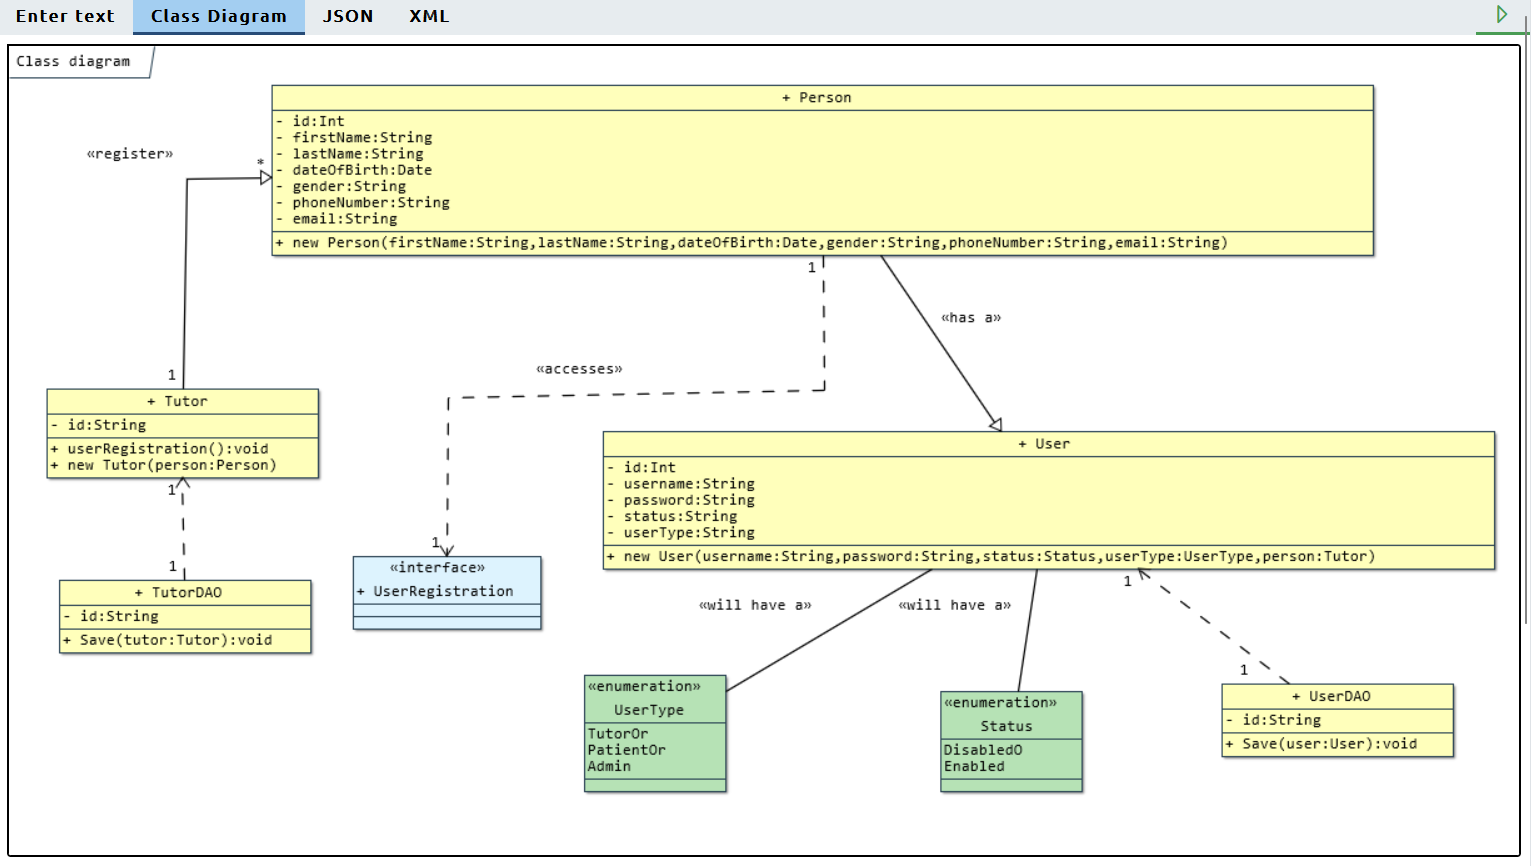
\includegraphics[width=15cm]{img/prueba08.png}
		\label{fig:prueba08}
		\vspace{4mm}
		{\footnotesize \textbf{\\ FUENTE: INVESTIGACIÓN} \textbf{\\ ELABORADO: AUTOR}}
	\end{figure}

	\item \textbf{Descripción \#9:}
	\begin{lstlisting}
		 Este caso de uso finaliza cuando el sistema muestra la interfaz de *(@/Login/). *¡Login u<[]<u UserDAO! \end{lstlisting}
	
	Finalmente, la descripción del caso de uso genera una interfaz que se denomina Login. Además está relacionada por medio del tipo Dependencia con la clase UserDAO (ver ilustración \ref{fig:prueba09}).
	
	\begin{lstlisting}
		Este caso de uso finaliza cuando el sistema muestra la interfaz de Login.\end{lstlisting}
	
	\begin{figure}[h!]
		\centering
		\caption{Diagrama de clases generado por la aplicación web de demostración usando la librería de armadillo.js, descripción 9}
		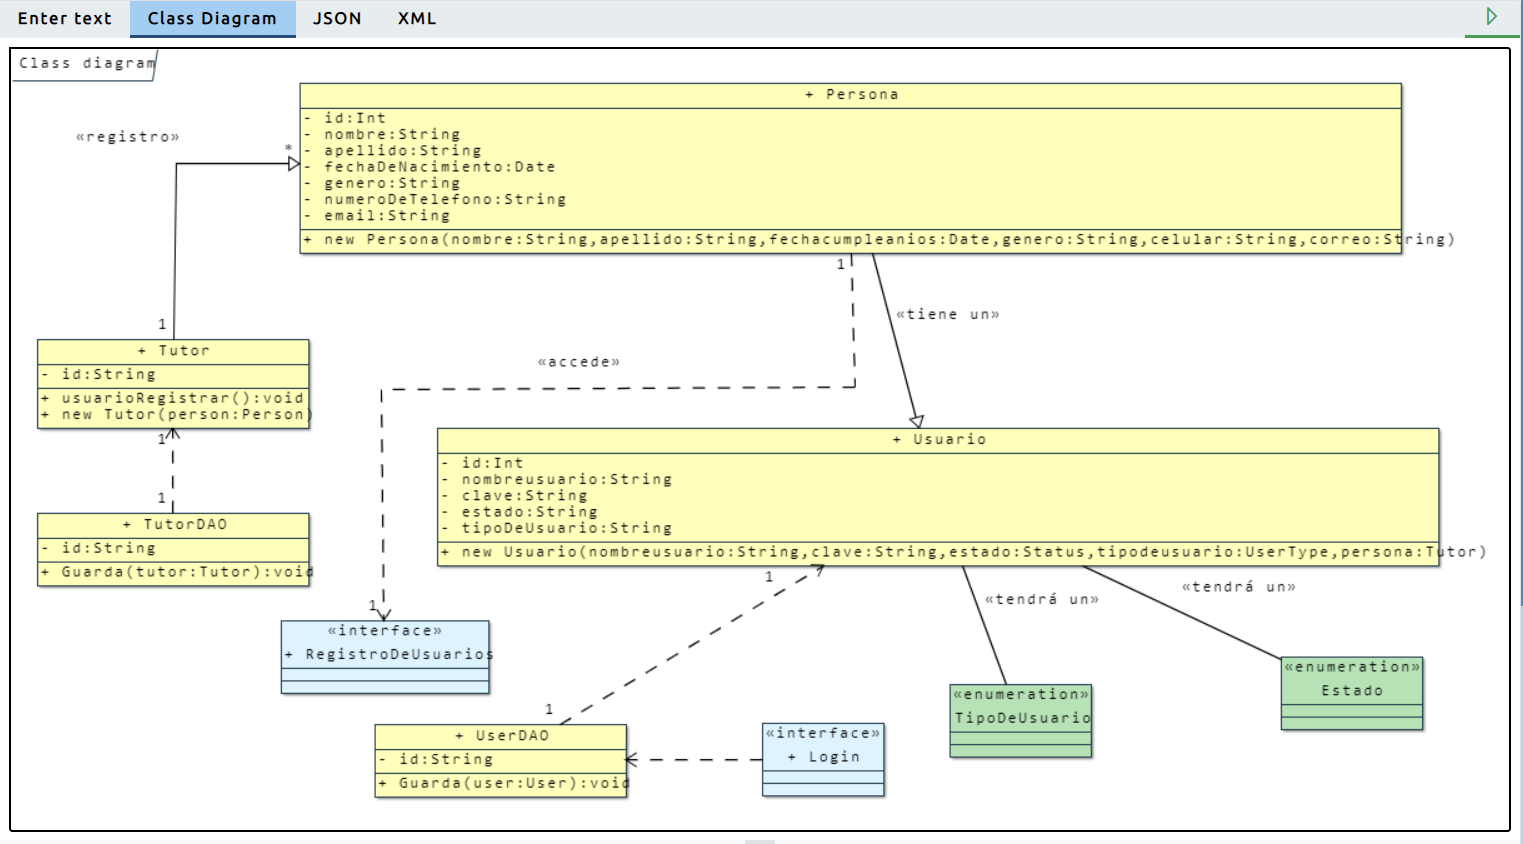
\includegraphics[width=15cm]{img/prueba09.png}
		\label{fig:prueba09}
		\vspace{4mm}
		{\footnotesize \textbf{\\ FUENTE: INVESTIGACIÓN} \textbf{\\ ELABORADO: AUTOR}}
	\end{figure}
	
\end{itemize}

Si se compara el diagrama de clases que fue recopilado en la primera fase de la metodología con el diagrama de clases generado mediante la librería. Se logra observar que son muy similares, y fue generado mediante las descripciones del caso de uso que fueron redactadas usando el lenguaje de símbolos.

\subsection{Evaluación con sistemas de información}

Para la ejecución de la fase final de la metodología se revisaron varios proyectos de titulación realizados por estudiantes de la Universidad Técnica Estatal de Quevedo. Se analizaron los sistemas desarrollados reescribiendo las descripciones de los casos de uso utilizando el lenguaje de símbolos.

En \cite{Villafuerte2020} se analizó el proyecto de titulación "SISTEMA BASADO EN INTERNET DE LAS COSAS PARA LA GESTIÓN DE LOS RECURSOS DE UN AULA DE CLASES" que fue realizado en la Universidad Técnica Estatal de Quevedo. Para empezar con el análisis se revisó el diagrama de casos de uso, seleccionando algunos casos de uso para realizar la respectiva evaluación de la librería. 

El objetivo de esta prueba es retroalimentar lo que se genera al interpretar cada descripción y comparar el diagrama de clases generado con el original del proyecto. En la ilustración \ref{fig:dcu_aula_inteligente} se observa el diagrama de casos de uso realizado por el proyecto de titulación. Para la evaluación se seleccionaron los casos: ingresar al sistema, solicitar accesos físicos temporales, acceder a cursos temporales, registrar asistencia de estudiantes.

\begin{figure}[h!]
	\centering
	\caption{Diagrama de casos de uso para "SISTEMA BASADO EN INTERNET DE LAS COSAS PARA LA GESTIÓN DE LOS RECURSOS DE UN AULA DE CLASES"}
	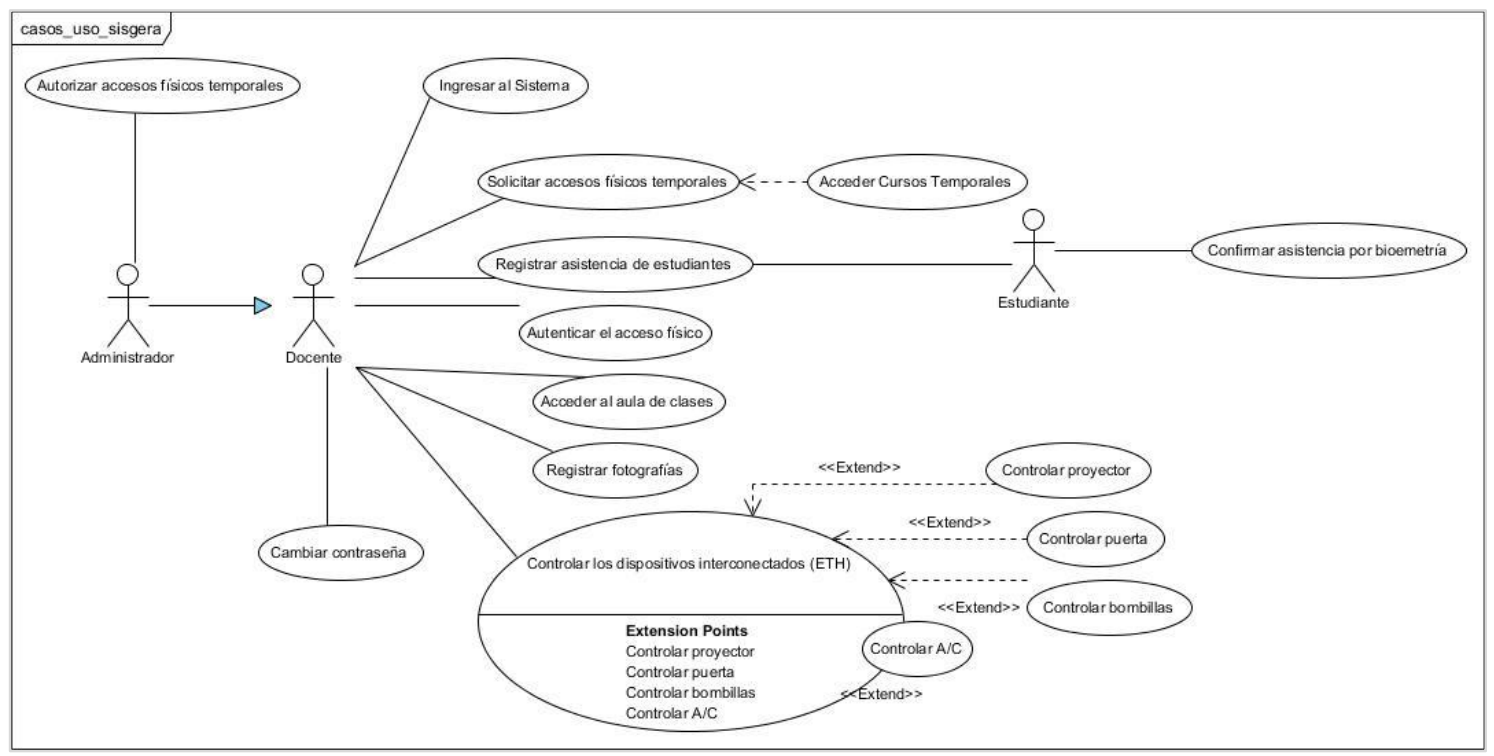
\includegraphics[width=13cm]{img/dgcu-aula-int.png}
	\label{fig:dcu_aula_inteligente}
	\vspace{4mm}
	{\footnotesize \textbf{\\ FUENTE:  VILLAFUERTE y YÁNEZ \cite{Villafuerte2020}}}
\end{figure}

Para mejorar la presentación de los casos de uso a evaluar, se realizó un diagrama de casos de uso con los seleccionados. Además, se redactaron las descripciones de cada caso de uso en 2 formas. La primera es con el texto natural detallando paso a paso las acciones que se deben realizar. La Segunda forma en como están representados los casos de uso es mediante el lenguaje de símbolos.

\begin{figure}[h!]
	\centering
	\caption{Diagrama de casos de uso basado en el "SISTEMA BASADO EN INTERNET DE LAS COSAS PARA LA GESTIÓN DE LOS RECURSOS DE UN AULA DE CLASES" para ser evaluado por armadillo.js}
	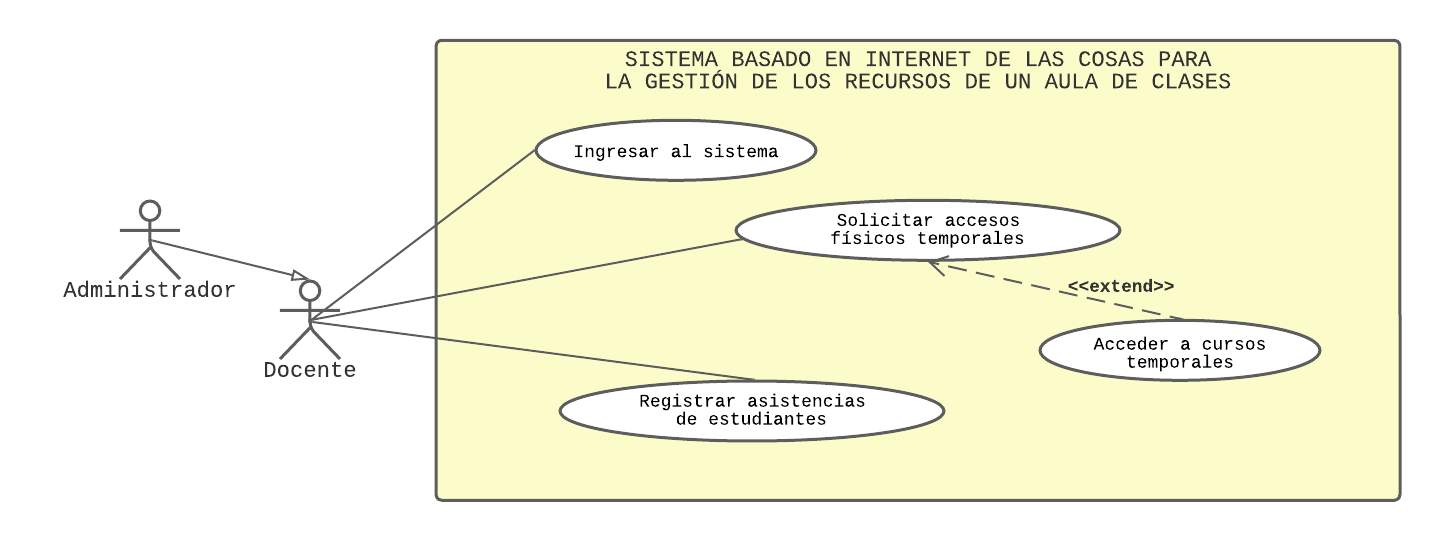
\includegraphics[width=15cm]{img/dcu_eva_ai.png}
	\label{fig:dcu_eva_aula_inteligente}
	\vspace{4mm}
	{\footnotesize \textbf{\\ FUENTE: VILLAFUERTE y YÁNEZ \cite{Villafuerte2020}} \textbf{\\ ELABORADO: AUTOR}}
\end{figure}

\begin{figure}[h!]
	\centering
	\caption{Diagrama de clases de el "SISTEMA BASADO EN INTERNET DE LAS COSAS PARA LA GESTIÓN DE LOS RECURSOS DE UN AULA DE CLASES" para ser evaluado por armadillo.js}
	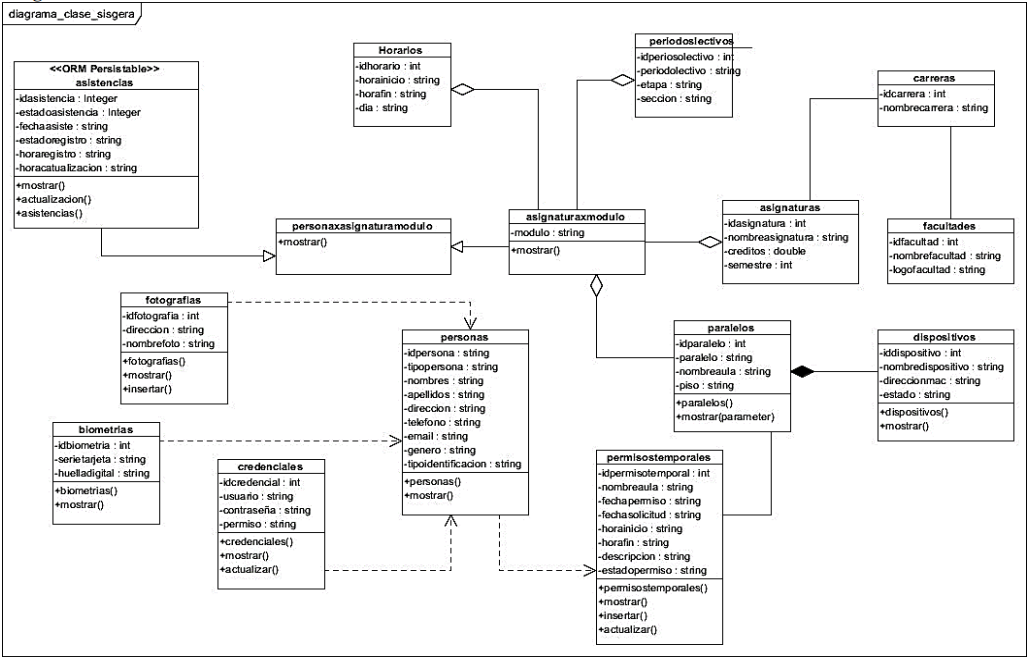
\includegraphics[width=13cm]{img/dclases-ai.png}
	\label{fig:dc_aula_inteligente}
	\vspace{4mm}
	{\footnotesize \textbf{\\ FUENTE: VILLAFUERTE y YÁNEZ \cite{Villafuerte2020}}}
\end{figure}

En la ilustración \ref{fig:dc_aula_inteligente} se observa el diagrama de clases para el sistema de información a analizar. En la fase de evaluación de la librería se tratará de generar un diagrama de clases lo más parecido posible al diagrama original. Además de indicar los errores si es que son cometidos al momento de redactar las descripciones de los casos de uso. 

A continuación en las tablas [\ref{tab:is_ai}, \ref{tab:sa_ai}, \ref{tab:ac_ai} \ref{tab:rae_ai}] se redactan las descripciones de los casos de uso seleccionados en lenguaje natural. En las tablas [\ref{tab:is_is_ls}, \ref{tab:aft_ai_ls}, \ref{tab:ac_ai_ls}, \ref{tab:rae_ai_ls}] se redactaron las descripciones de los casos de uso usando el lenguaje de símbolos.

Para evaluar las descripciones de los casos de uso se detallará cada descripción con su respectiva retroalimentación y como se va modificando el diagrama de clases conforme se ingresan más descripciones.

\begin{lstlisting}[]
	1. El actor docente o administrador *(persona) ingresará las *(credenciales) credenciales proporcionadas por la institución, estas se validarán y posterior otorgará el acceso a las opciones. \end{lstlisting}

\begin{figure}[h!]
	\centering
	\caption{Mensajes de consola relacionado a la escritura de la descripción 1.}
	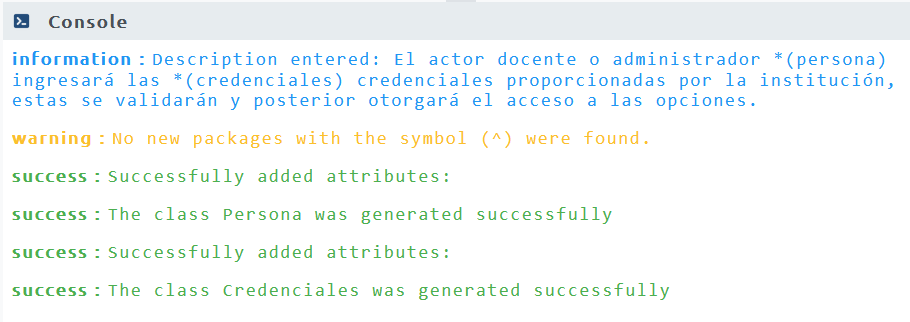
\includegraphics[width=12cm]{img/not-eva-001.png}
	\label{fig:not_eva_001}
	\textbf{\\ ELABORADO: DÚVAL CARVAJAL SUÁREZ}
\end{figure}

\begin{figure}[H]
	\centering
	\caption{Diagrama de clases generado para la descripción 1.}
	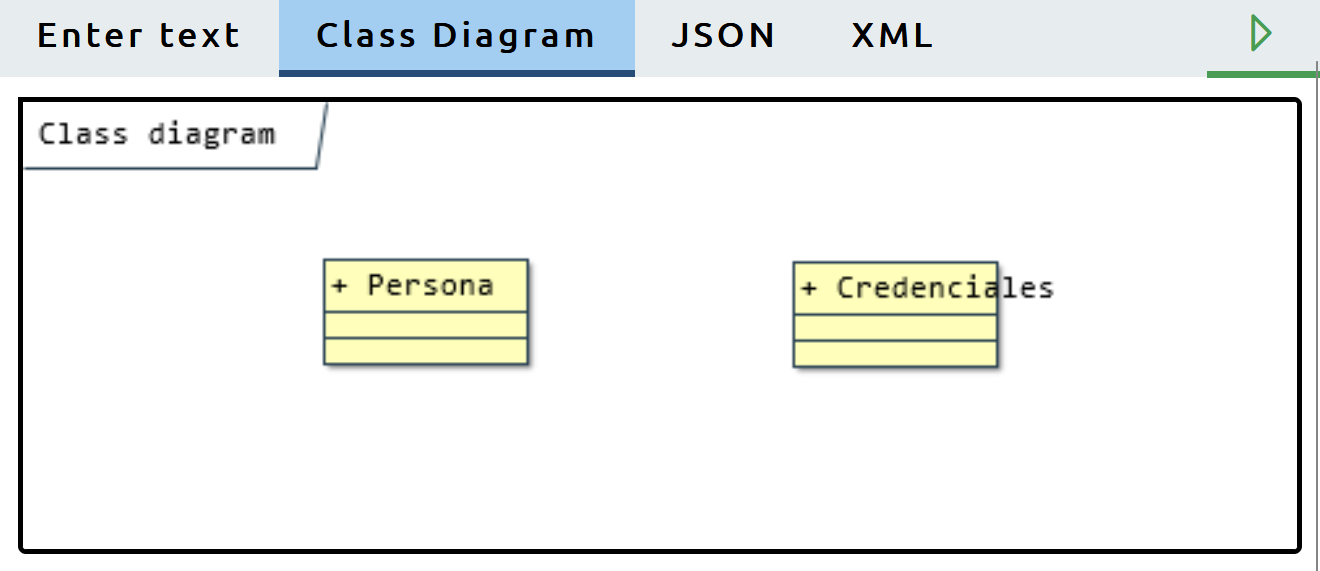
\includegraphics[width=10cm]{img/dc-eva-001.png}
	\label{fig:dc_eva_001}
	\vspace{4mm}
	{\footnotesize \textbf{\\ FUENTE:INVESTIGACIÓN} \textbf{\\ ELABORADO: AUTOR}}
\end{figure}

\begin{lstlisting}
	 2. El caso de uso se inicia cuando el actor docente o administrador *(persona &-id=string &-tipo=string &-nombres=string &-apellidos=string &-direccion=string &-telefono=string &-email=string &-genero = string &-tipoidentificion=string [+persona=empty] [+mostrar=empty]) necesita acceder a la aplicación, para ello ingresa a la aplicación móvil en su dispositivo smartphone. \end{lstlisting}
 
 \begin{figure}[h!]
 	\centering
 	\caption{Mensajes de consola relacionado a la escritura de la descripción 2.}
 	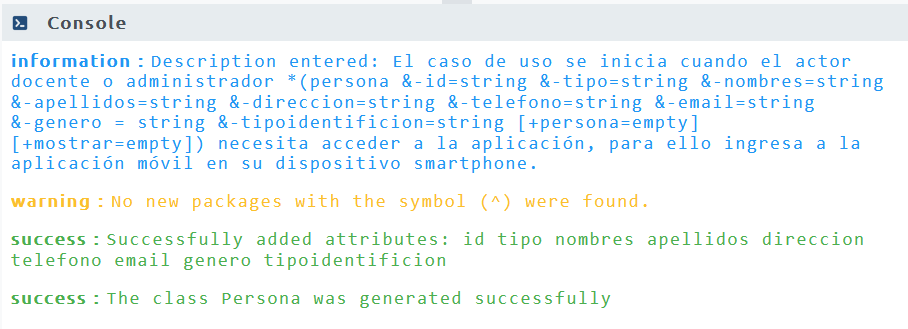
\includegraphics[width=14cm]{img/not-eva-002.png}
 	\label{fig:not_eva_002}
 	\vspace{4mm}
 	{\footnotesize \textbf{\\ FUENTE: INVESTIGACIÓN} \textbf{\\ ELABORADO: AUTOR}}
 \end{figure}
 
 \begin{figure}[H]
 	\centering
 	\caption{Diagrama de clases generado para la descripción 2.}
 	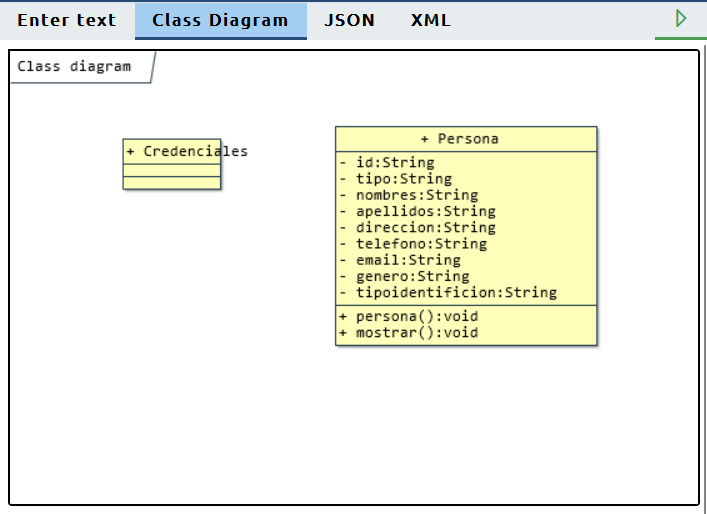
\includegraphics[width=10cm]{img/dc-eva-002.png}
 	\label{fig:dc_eva_002}
 	\vspace{4mm}
 	{\footnotesize \textbf{\\ FUENTE:INVESTIGACIÓN} \textbf{\\ ELABORADO: AUTOR}}
 \end{figure}
 
 \begin{lstlisting}
 	3. El actor docente o administrador ingresa el *(credenciales &-id=int &-/usuario/=String /y/ &-/contraseña/=String &-permiso=string [+credenciales=empyt] [+mostrar=empty] [+actualizar=empty]) asignados por la institución; y da clic en el botón Ingresar. *¡persona 1<[tiene]<1 credenciales! \end{lstlisting}
 
  \begin{figure}[h!]
  	\centering
 	\caption{Mensajes de consola notificando si existe algún error en la escritura de la descripción 3.}
 	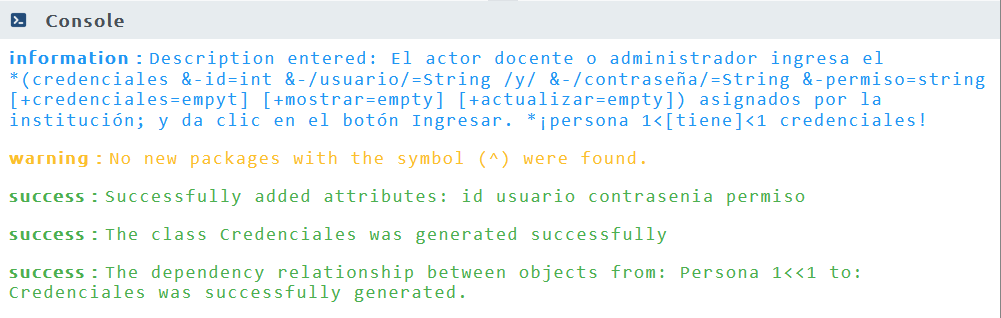
\includegraphics[width=14cm]{img/not-eva-003.png}
 	\label{fig:not_eva_003}
 	\vspace{4mm}
 	{\footnotesize \textbf{\\ FUENTE: INVESTIGACIÓN} \textbf{\\ ELABORADO: AUTOR}}
 \end{figure}
 
 \begin{figure}[H]
 	\centering
 	\caption{Diagrama de clases generado para la descripción 3.}
 	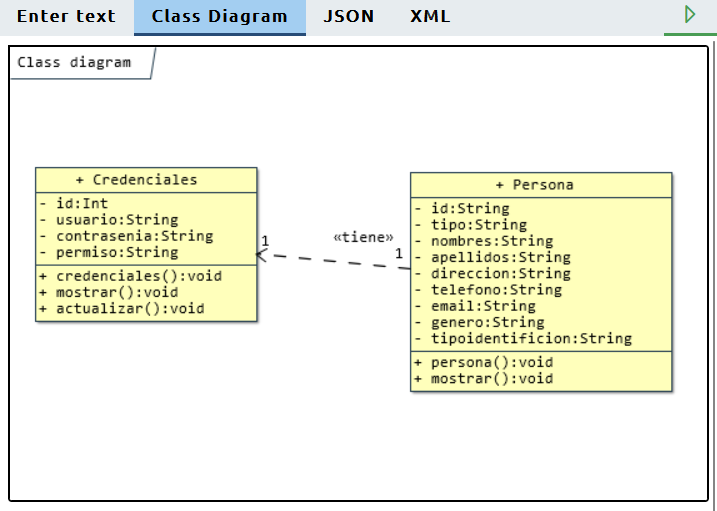
\includegraphics[width=10cm]{img/dc-eva-003.png}
 	\label{fig:dc_eva_003}
 	\vspace{4mm}
 	{\footnotesize \textbf{\\ FUENTE: INVESTIGACIÓN} \textbf{\\ ELABORADO: AUTOR}}
 \end{figure}
 
  \begin{lstlisting}
 	4. El caso de uso se inicia cuando el docente necesita tener acceso temporalmente *(permisos temporales [+permisosTemporales=empyt] [+mostrar=empty] [+insertar=empty] [+actualizar=empty]) a un aula de clases que se encuentre disponible no utilizada. \end{lstlisting}
 
   \begin{figure}[h!]
   	\centering
 	\caption{Mensajes de consola relacionado a la escritura de la descripción 4.}
 	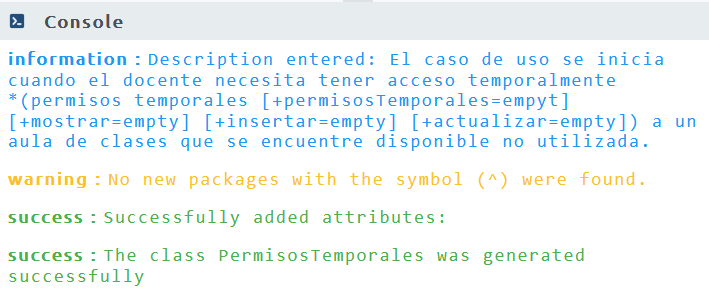
\includegraphics[width=14cm]{img/not-eva-004.png}
 	\label{fig:not_eva_004}
 	\vspace{4mm}
 	{\footnotesize \textbf{\\ FUENTE: INVESTIGACIÓN} \textbf{\\ ELABORADO: AUTOR}}
 \end{figure}
 
 \begin{figure}[H]
 	\centering
 	\caption{Diagrama de clases generado para la descripción 4.}
 	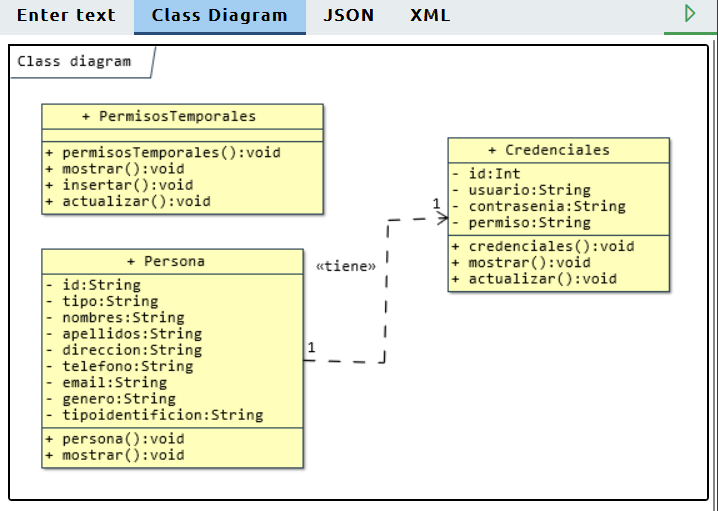
\includegraphics[width=10cm]{img/dc-eva-004.png}
 	\label{fig:dc_eva_004}
 	\vspace{4mm}
 	{\footnotesize \textbf{\\ FUENTE: INVESTIGACIÓN} \textbf{\\ ELABORADO: AUTOR}}
 \end{figure}
 
 \begin{lstlisting}
 	5. El docente llenará la información solicitada por la interfaz, que consiste en el curso a solicitar, la *(permisos temporales &-id=int &-nombreaula &-/fecha del permiso/=string /que requiere el acceso,/ &-fecha de la solicitud=string &-/hora de inicio/=string /y/ &-/hora de fin/=string /del permiso; y, una/ &-/descripción/=string &-estado=string) donde detallará brevemente la justificación del permiso. Una vez culminado, dará clic en el botón Enviar. *¡persona 1<[podra solicitar]<1 permisos temporales! \end{lstlisting}
 
    \begin{figure}[h!]
    	\centering
 	\caption{Mensajes de consola relacionado a la escritura de la descripción 5.}
 	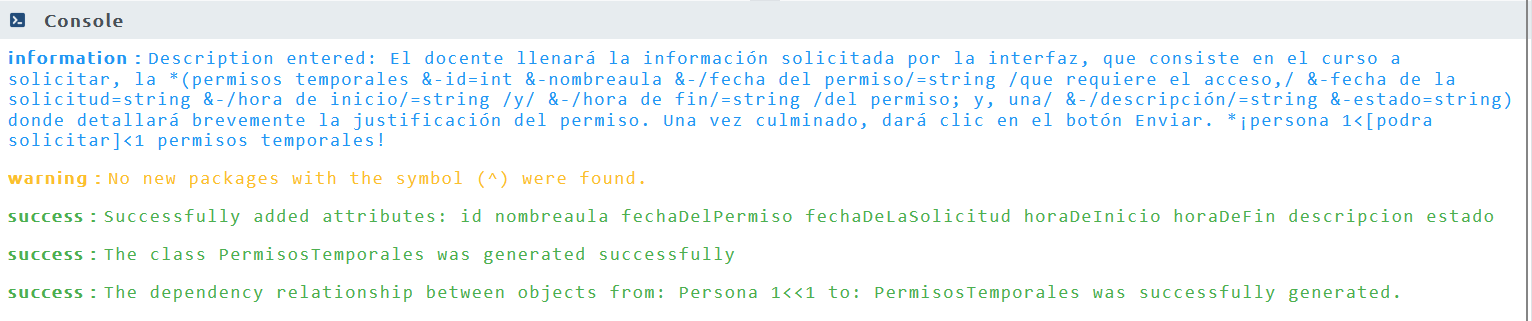
\includegraphics[width=15cm]{img/not-eva-005.png}
 	\label{fig:not_eva_005}
 	\vspace{4mm}
 	{\footnotesize \textbf{\\ FUENTE: INVESTIGACIÓN} \textbf{\\ ELABORADO: AUTOR}}
 \end{figure}
 
 \begin{figure}[H]
 	\centering
 	\caption{Diagrama de clases generado para la descripción 5.}
 	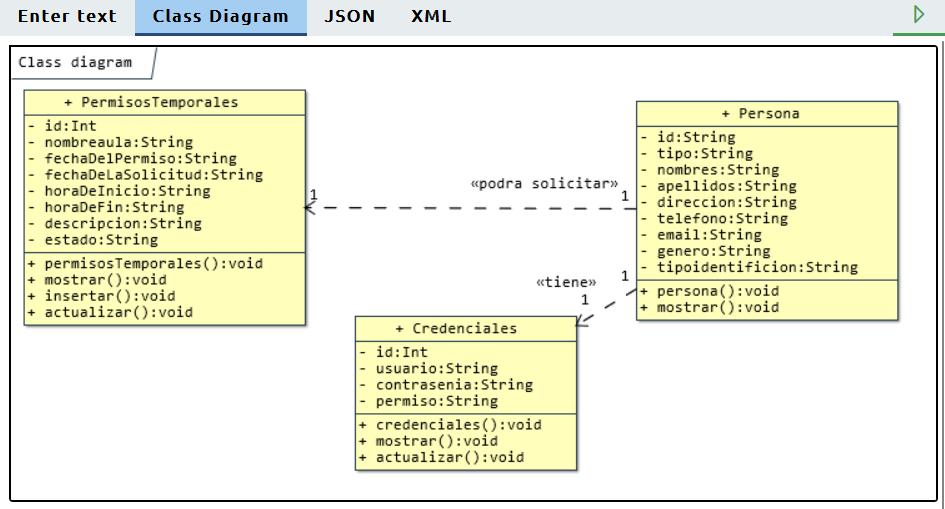
\includegraphics[width=15cm]{img/dc-eva-005.png}
 	\label{fig:dc_eva_005}
 	\vspace{4mm}
 	{\footnotesize \textbf{\\ FUENTE: INVESTIGACIÓN} \textbf{\\ ELABORADO: AUTOR}}
 \end{figure}
 
 \begin{lstlisting}
 	6. Ingresar al aula de clases *(paralelos &-id=int &-paralelo=string &-nombreaula=string &-piso=string [+paralelos=empty] [+mostrar=empty]) que el docente solicitó un permiso temporal, previo a la autorización del administrador \end{lstlisting}
 
    \begin{figure}[h!]
    	\centering
 	\caption{Mensajes de consola relacionado a la escritura de la descripción 6.}
 	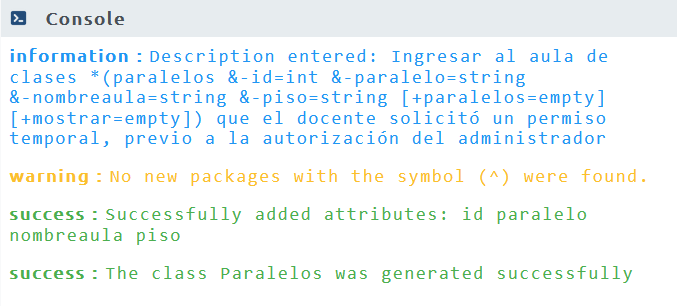
\includegraphics[width=10cm]{img/not-eva-006.png}
 	\label{fig:not_eva_006}
 	\vspace{4mm}
 	{\footnotesize \textbf{\\ FUENTE: INVESTIGACIÓN} \textbf{\\ ELABORADO: AUTOR}}
 \end{figure}
 
 \begin{figure}[H]
 	\centering
 	\caption{Diagrama de clases generado para la descripción 6.}
 	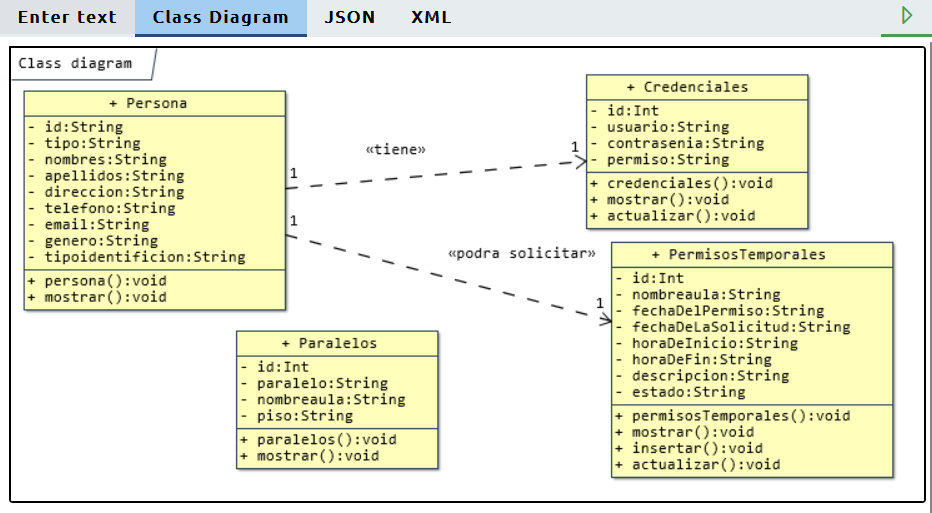
\includegraphics[width=15cm]{img/dc-eva-006.png}
 	\label{fig:dc_eva_006}
 	\vspace{4mm}
 	{\footnotesize \textbf{\\ FUENTE: INVESTIGACIÓN} \textbf{\\ ELABORADO: AUTOR}}
 \end{figure}
 
  \begin{lstlisting}
 	7. Acceso al curso temporal en la aplicación móvi  luego de obtener autorización, donde podrá manipular los dispositivos *(dispositivos &-id=int &-nombre=string &-direccionmac &-estado=string [+dispositivos=empty] [+mostrar=empty]) eléctricos y electrónicos ETH. \end{lstlisting}
 
     \begin{figure}[h!]
     	\centering
 	\caption{Mensajes de consola relacionado a la escritura de la descripción 7.}
 	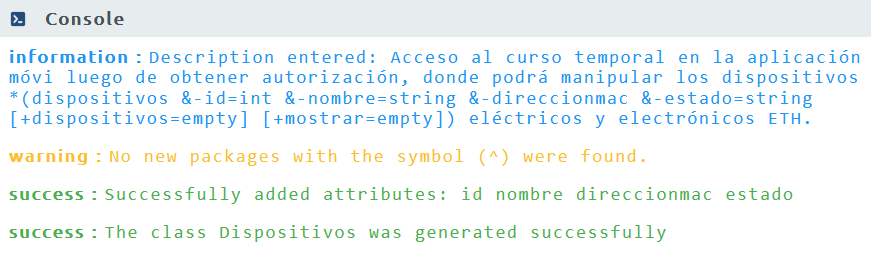
\includegraphics[width=14cm]{img/not-eva-007.png}
 	\label{fig:not_eva_007}
 	\vspace{4mm}
 	{\footnotesize \textbf{\\ FUENTE: INVESTIGACIÓN} \textbf{\\ ELABORADO: AUTOR}}
 \end{figure}
 
 \begin{figure}[H]
 	\centering
 	\caption{Diagrama de clases generado para la descripción 7.}
 	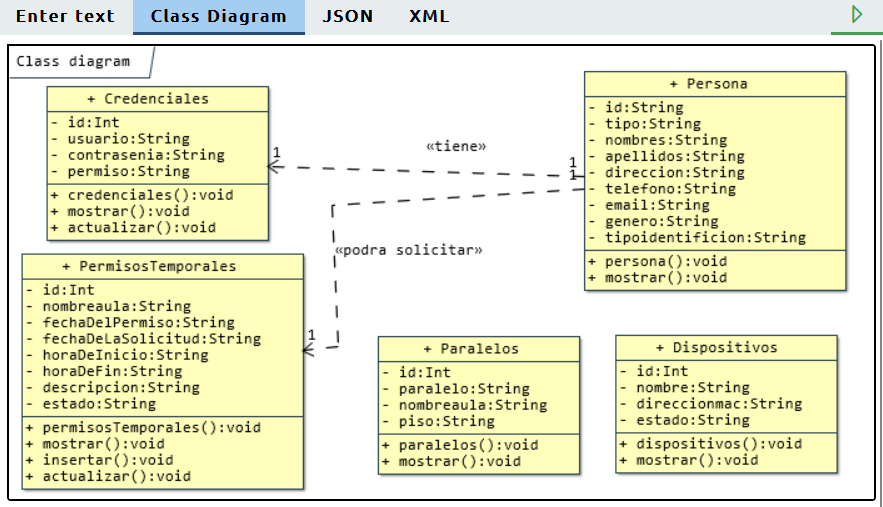
\includegraphics[width=15cm]{img/dc-eva-007.png}
 	\label{fig:dc_eva_007}
 	\vspace{4mm}
 	{\footnotesize \textbf{\\ FUENTE: INVESTIGACIÓN} \textbf{\\ ELABORADO: AUTOR}}
 \end{figure}
 
 \begin{lstlisting}
 	8. El caso de uso se inicia cuando el docente *¡permisos temporales 1<[/accede temporalmente/]>n paralelos! a un aula de clases que se encuentre disponible, es decir no utilizada.
 \end{lstlisting}

     \begin{figure}[h!]
     	\centering
	\caption{Mensajes de consola relacionado a la escritura de la descripción 8.}
	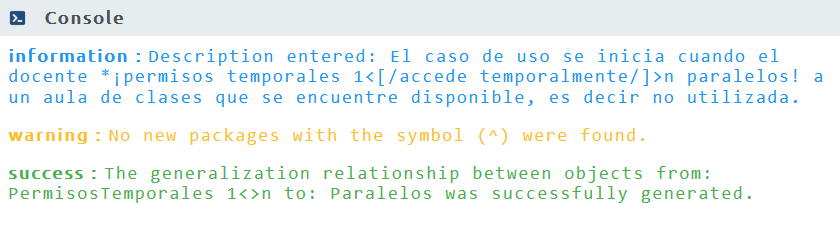
\includegraphics[width=14cm]{img/not-eva-008.png}
	\label{fig:not_eva_008}
	\vspace{4mm}
	{\footnotesize \textbf{\\ FUENTE: INVESTIGACIÓN} \textbf{\\ ELABORADO: AUTOR}}
\end{figure}

\begin{figure}[H]
	\centering
	\caption{Diagrama de clases generado para la descripción 8.}
	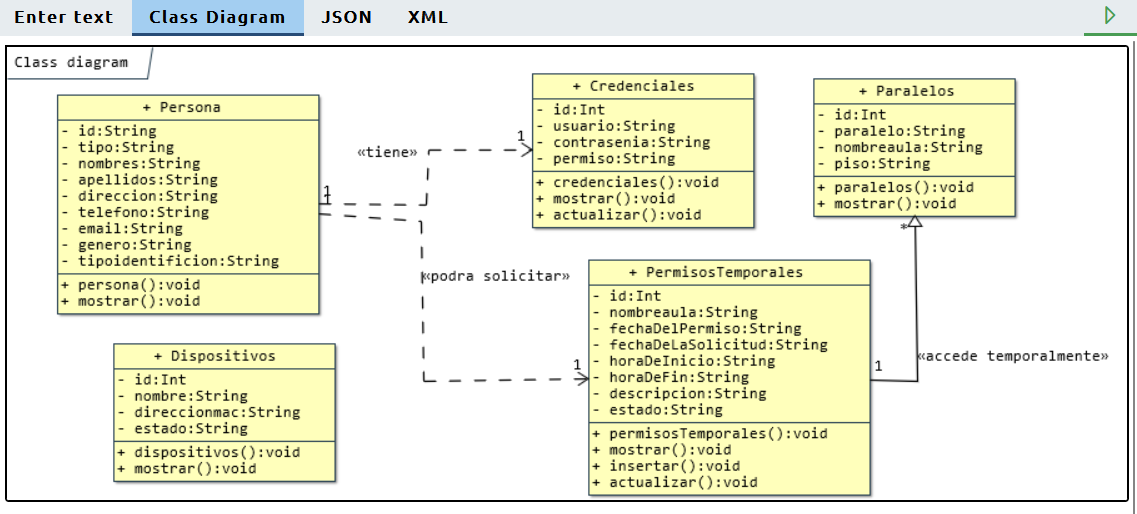
\includegraphics[width=15cm]{img/dc-eva-008.png}
	\label{fig:dc_eva_008}
	\vspace{4mm}
	{\footnotesize \textbf{\\ FUENTE: INVESTIGACIÓN} \textbf{\\ ELABORADO: AUTOR}}
\end{figure}

\begin{lstlisting}
	 9. El docente acepta la vinculación, accede al curso y  *¡paralelos 1<[/tiene control de los/]<n dispositivos! eléctricos y electrónicos ETH. Quedando concluido el caso de uso.
\end{lstlisting}

     \begin{figure}[h!]
     	\centering
	\caption{Mensajes de consola relacionado a la escritura de la descripción 9.}
	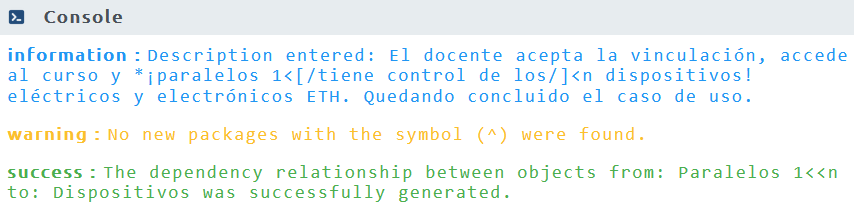
\includegraphics[width=14cm]{img/not-eva-009.png}
	\label{fig:not_eva_009}
	\vspace{4mm}
	{\footnotesize \textbf{\\ FUENTE: INVESTIGACIÓN} \textbf{\\ ELABORADO: AUTOR}}
\end{figure}

\begin{figure}[H]
	\centering
	\caption{Diagrama de clases generado para la descripción 9.}
	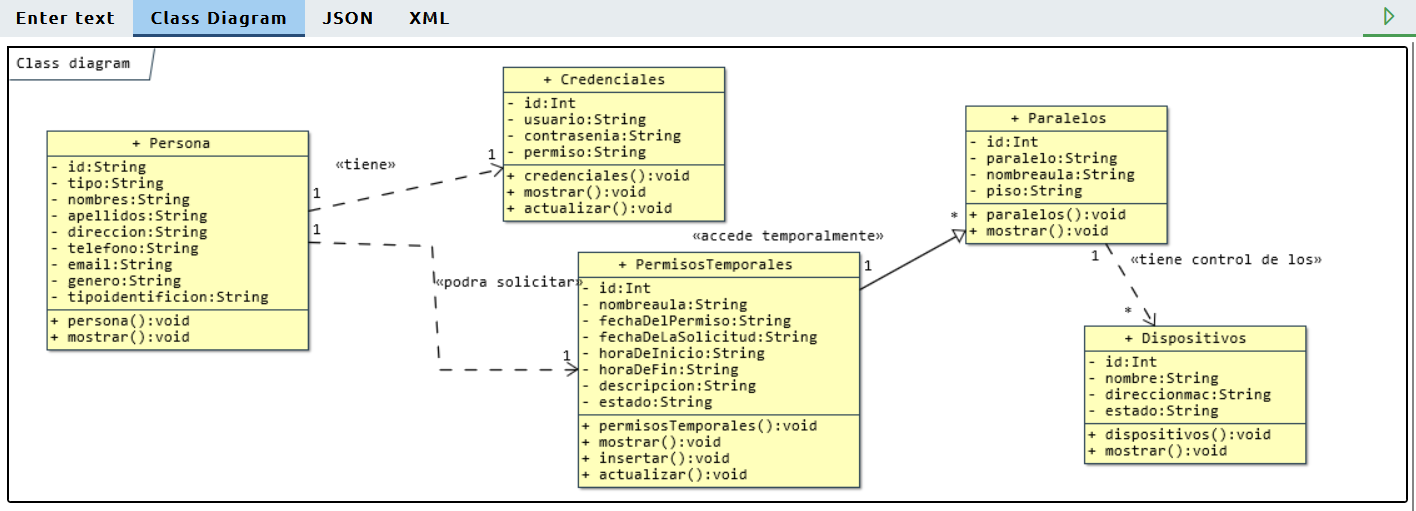
\includegraphics[width=15cm]{img/dc-eva-009.png}
	\label{fig:dc_eva_009}
	\vspace{4mm}
	{\footnotesize \textbf{\\ FUENTE: INVESTIGACIÓN} \textbf{\\ ELABORADO: AUTOR}}
\end{figure}

\begin{lstlisting}
	10. Posterior a la autenticación facial del docente, los estudiantes ingresarán al curso colocando su credencial *(biometrías &-id=int &-serietarjeta=string &-huelladigital=string [+biometrias=empty] [+mostrar=empty]) especial por el Lector RFID, luego el docente ingresará a la aplicación, validará el registro temporal de asistencias y enviará estas asistencias a almacenarse en la base de datos. *¡persona 1<[tiene]<n biometrías!
\end{lstlisting}

     \begin{figure}[h!]
     	\centering
	\caption{Mensajes de consola relacionado a la escritura de la descripción 10.}
	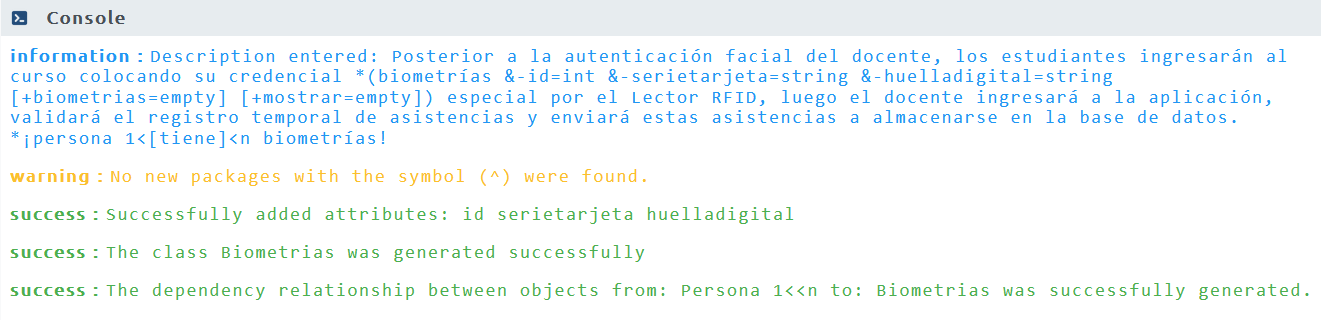
\includegraphics[width=14cm]{img/not-eva-010.png}
	\label{fig:not_eva_010}
	\vspace{4mm}
	{\footnotesize \textbf{\\ FUENTE: INVESTIGACIÓN} \textbf{\\ ELABORADO: AUTOR}}
\end{figure}

\begin{figure}[H]
	\centering
	\caption{Diagrama de clases generado para la descripción 10.}
	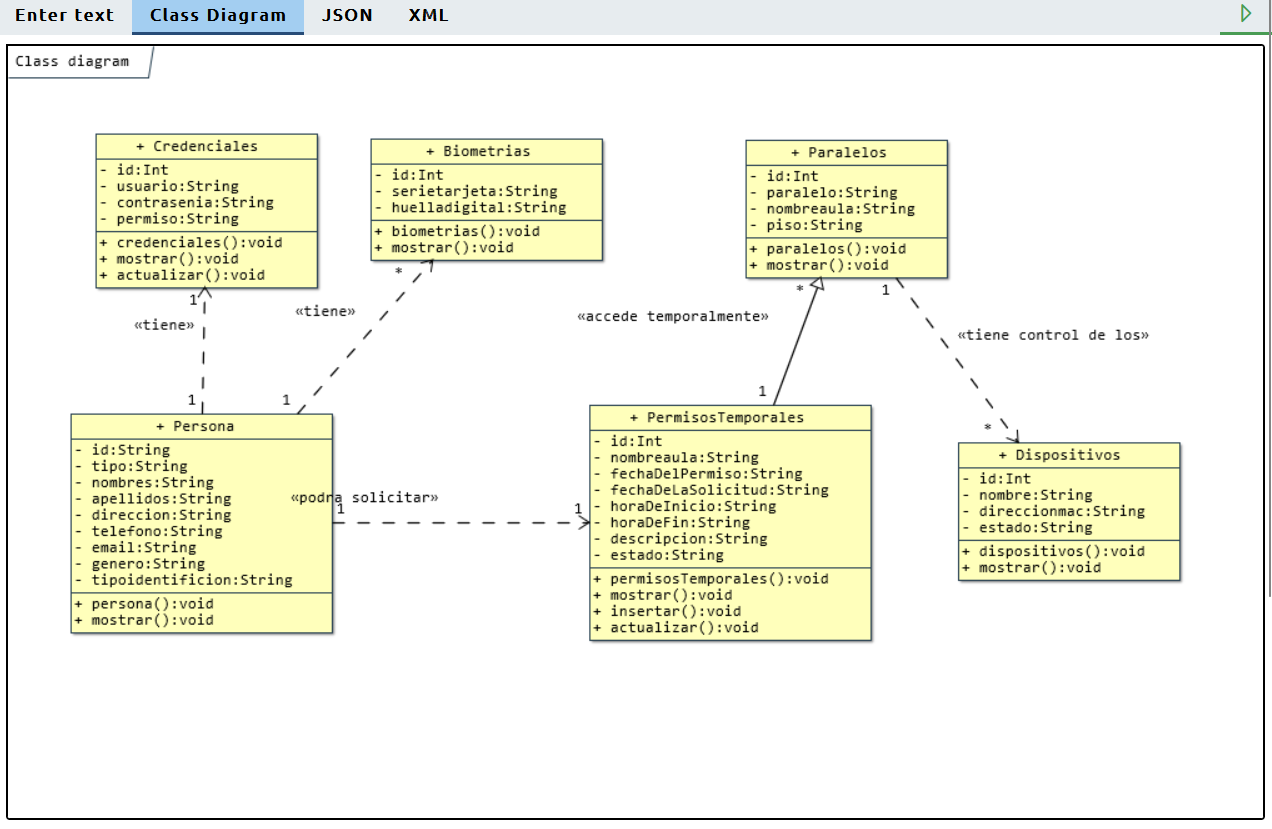
\includegraphics[width=15cm]{img/dc-eva-010.png}
	\label{fig:dc_eva_010}
	\vspace{4mm}
	{\footnotesize \textbf{\\ FUENTE: INVESTIGACIÓN} \textbf{\\ ELABORADO: AUTOR}}
\end{figure}

\begin{lstlisting}
	11. El caso de uso se inicia cuando el docente va a impartir su cátedra en el curso asignado, para ello posterior a su autenticación facial *(fotografías &-id=int &-direccion=string &-nombrefoto=string [+fotografias=empty] [+mostrar=empty] [+insertar=empty]), ingresará a curso acompañado de los estudiantes asignados *¡persona 1<[tiene]>n fotografías! a dicha materia.
\end{lstlisting}

     \begin{figure}[h!]
     	\centering
	\caption{Mensajes de consola relacionado a la escritura de la descripción 11.}
	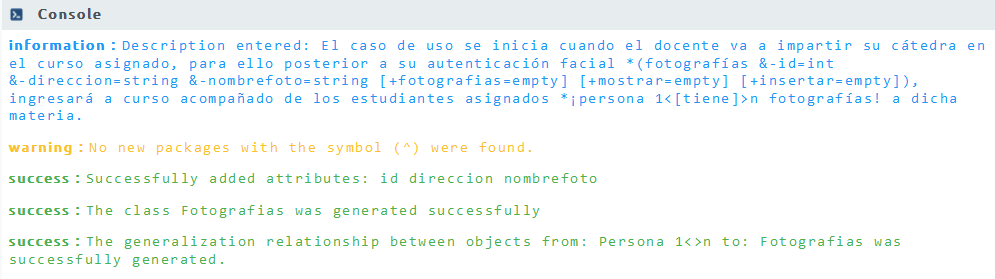
\includegraphics[width=14cm]{img/not-eva-011.png}
	\label{fig:not_eva_011}
	\vspace{4mm}
	{\footnotesize \textbf{\\ FUENTE: INVESTIGACIÓN} \textbf{\\ ELABORADO: AUTOR}}
\end{figure}

\begin{figure}[H]
	\centering
	\caption{Diagrama de clases generado para la descripción 10.}
	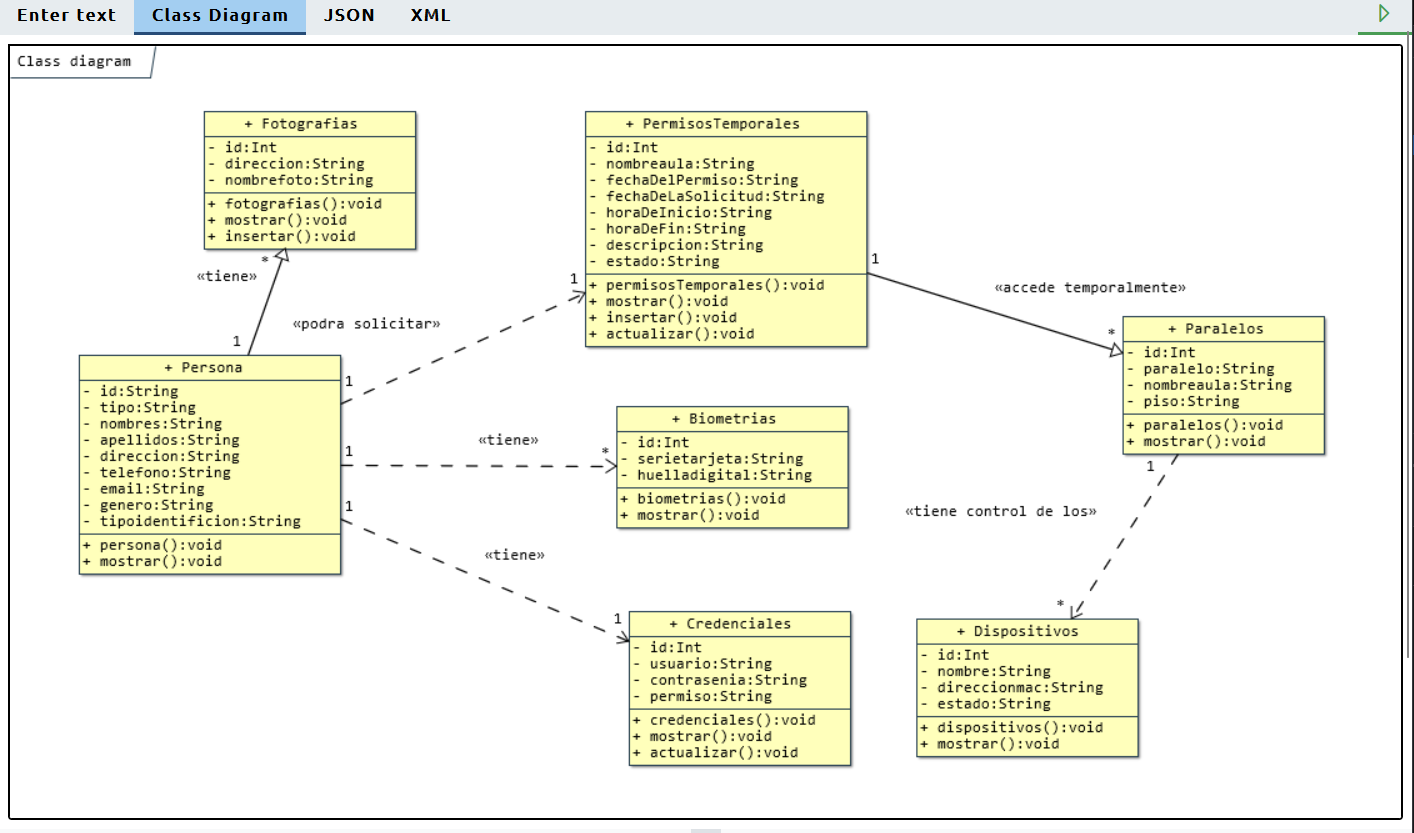
\includegraphics[width=15cm]{img/dc-eva-011.png}
	\label{fig:dc_eva_011}
	\vspace{4mm}
	{\footnotesize \textbf{\\ FUENTE: INVESTIGACIÓN} \textbf{\\ ELABORADO: AUTOR}}
\end{figure}

El diagrama de clases que se observa el ilustración \ref{fig:dc_eva_011} es el diagrama final que se obtiene luego de ingresar todas las descripciones de los casos de uso. Si se compara con el original se han generado varias clases iguales a las del diagrama de clases original. También se observan los mensajes de retroalimentación que sucede al momento de interpretar cada una de las descripciones.

\begin{table}[h!]
	\centering
	\caption{Descripción del caso de uso para ingresar al sistema.}
	\label{tab:is_ai}
	\begin{tabular}{| p{3cm} | p{11cm} |}
		\hline
		\textbf{Caso de uso:} & Ingresar al sistema \\ \hline
		\textbf{Actores:} & Docente, Administrador \\ \hline
		\textbf{Propósito:} & Acceder a la aplicación móvil para obtener las diversas opciones que permite el control del curso. \\ \hline
		\textbf{Resumen:} & El actor docente o administrador ingresará las credenciales proporcionadas por la institución, estas se validarán y posterior otorgará el acceso a las opciones.  \\ \hline
		\textbf{Tipo:} & Primario \\ \hline
		\multicolumn{2}{ |c| }{\textbf{Flujo normal}} \\ \hline
	\end{tabular}
	\begin{tabular}{| p{7cm} | p{7cm} |}
		\textbf{Acción del actor} & \textbf{Respuesta del sistema} \\ \hline	
		1. El caso de uso se inicia cuando el actor docente o administrador necesita acceder a la aplicación, para ello ingresa a la aplicación móvil en su dispositivo smartphone.  & \\ \hline
		& 2. Muestra el formulario correspondiente. \\ \hline
		3. El actor docente o administrador ingresa el usuario y contraseña asignados por la institución; y da clic en el botón Ingresar. & \\ \hline
		&4. Válida que los datos sean correctos y muestra el formulario de la ventana principal, dando por concluido el caso de uso. \\ \hline
		\multicolumn{2}{ |c| }{\textbf{Flujos alternos}} \\ \hline
	\end{tabular}
	\begin{tabular}{| p{7cm} | p{7cm} |}
		\textbf{Acción del actor} & \textbf{Respuesta del sistema} \\ \hline	
		& 4.1 Muestra un mensaje de credenciales incorrectas y retorne a la línea 2.  \\ \hline
	\end{tabular}
	\vspace{4mm}
	{\footnotesize \textbf{\\ FUENTE: INVESTIGACIÓN} \textbf{\\ ELABORADO: AUTOR}}
\end{table}

\begin{table}[h!]
	\centering
	\caption{Descripción del caso de uso con Symlen para ingresar al sistema.}
	\label{tab:is_is_ls}
	\begin{tabular}{| p{3cm} | p{11cm} |}
		\hline
		\textbf{Caso de uso:} & Ingresar al sistema \\ \hline
		\textbf{Actores:} & Docente, Administrador \\ \hline
		\textbf{Propósito:} & Acceder a la aplicación móvil para obtener las diversas opciones que permite el control del curso. \\ \hline
		\textbf{Resumen:} & El actor docente o administrador *(persona) ingresará las *(credenciales) credenciales proporcionadas por la institución, estas se validarán y posterior otorgará el acceso a las opciones.  \\ \hline
		\textbf{Tipo:} & Primario \\ \hline
		\multicolumn{2}{ |c| }{\textbf{Flujo normal}} \\ \hline
	\end{tabular}
	\begin{tabular}{| p{7cm} | p{7cm} |}
		\textbf{Acción del actor} & \textbf{Respuesta del sistema} \\ \hline	
		1. El caso de uso se inicia cuando el actor docente o administrador *(persona \&-id=string \&-tipo=string \&-nombres=string \&-apellidos=string \&-direccion=string \&-telefono=string \&-email=string \&-genero = string \&-tipoidentificion=string [+persona=empty] [+mostrar=empty]) necesita acceder a la aplicación, para ello ingresa a la aplicación móvil en su dispositivo smartphone.  & \\ \hline
		& 2. Muestra el formulario correspondiente. \\ \hline
		3.El actor docente o administrador ingresa el *(credenciales \&-id=int \&-/usuario/=String /y/ \&-/contraseña/=String \&-permiso=string [+credenciales=empyt] [+mostrar=empty] [+actualizar=empty]) asignados por la institución; y da clic en el botón Ingresar. *¡persona 1<[tiene]<1 credenciales! & \\ \hline
		&4. Válida que los datos sean correctos y muestra el formulario de la ventana principal, dando por concluido el caso de uso. \\ \hline
		\multicolumn{2}{ |c| }{\textbf{Flujos alternos}} \\ \hline
	\end{tabular}
	\begin{tabular}{| p{7cm} | p{7cm} |}
		\textbf{Acción del actor} & \textbf{Respuesta del sistema} \\ \hline	
		& 4.1 Muestra un mensaje de credenciales incorrectas y retorne a la línea 2.  \\ \hline
	\end{tabular}
	\vspace{4mm}
	{\footnotesize \textbf{\\ FUENTE: INVESTIGACIÓN} \textbf{\\ ELABORADO: AUTOR}}
\end{table}

\begin{table}[h!]
	\centering
	\caption{Descripción del caso de uso para solicitar accesos físicos temporales.}
	\label{tab:sa_ai}
	\begin{tabular}{| p{3cm} | p{11cm} |}
		\hline
		\textbf{Caso de uso:} & Solicitar accesos físicos temporales \\ \hline
		\textbf{Actores:} & Docente \\ \hline
		\textbf{Propósito:} & Solicitar acceso a un aula de clases en un tiempo determinado, teniendo en cuenta que está no se encuentre ocupada por otro docente. \\ \hline
		\textbf{Resumen:} & El docente dentro de la aplicación móvil, escogerá la opción “Permisos cursos” dentro del menú y llenará la información solicitada.  \\ \hline
		\textbf{Tipo:} & Primario \\ \hline
		\multicolumn{2}{ |c| }{\textbf{Flujo normal}} \\ \hline
	\end{tabular}
	\begin{tabular}{| p{7cm} | p{7cm} |}
		\textbf{Acción del actor} & \textbf{Respuesta del sistema} \\ \hline	
		1. El caso de uso se inicia cuando el docente necesita tener acceso temporalmente a un aula de clases que se encuentre disponible no utilizada.   & \\ \hline
		2. El docente, una vez autenticado en la aplicación móvil, ingresará al menú y escogerá la opción “Permisos cursos”.&\\ \hline
		& 3. Muestra el formulario correspondiente. \\ \hline
		4. El docente llenará la información solicitada por la interfaz, que consiste en el curso a solicitar, la fecha del permiso que requiere el acceso, hora de inicio y hora de fin del permiso; y, una descripción donde detallará brevemente la justificación del permiso. Una vez culminado, dará clic en el botón Enviar. &  \\ \hline
		& 5. Mostrará un mensaje de envío correcto de la información, finalizando el caso de uso. \\ \hline
		\multicolumn{2}{ |c| }{\textbf{Flujos alternos}} \\ \hline
	\end{tabular}
	\begin{tabular}{| p{7cm} | p{7cm} |}
		\textbf{Acción del actor} & \textbf{Respuesta del sistema} \\ \hline	
		& 5.1 : Muestra un mensaje de error y retorne a la línea 4.   \\ \hline
	\end{tabular}
	\vspace{4mm}
	{\footnotesize \textbf{\\ FUENTE: INVESTIGACIÓN} \textbf{\\ ELABORADO: AUTOR}}
\end{table}

\begin{table}[h!]
	\centering
	\caption{Descripción del caso de uso con Symlen para solicitar accesos físicos temp.}
	\label{tab:aft_ai_ls}
	\begin{tabular}{| p{3cm} | p{11cm} |}
		\hline
		\textbf{Caso de uso:} & Solicitar accesos físicos temporales \\ \hline
		\textbf{Actores:} & Docente \\ \hline
		\textbf{Propósito:} & Solicitar acceso a un aula de clases en un tiempo determinado, teniendo en cuenta que está no se encuentre ocupada por otro docente. \\ \hline
		\textbf{Resumen:} & El docente dentro de la aplicación móvil, escogerá la opción “Permisos cursos” dentro del menú y llenará la información solicitada.  \\ \hline
		\textbf{Tipo:} & Primario \\ \hline
		\multicolumn{2}{ |c| }{\textbf{Flujo normal}} \\ \hline
	\end{tabular}
	\begin{tabular}{| p{7cm} | p{7cm} |}
		\textbf{Acción del actor} & \textbf{Respuesta del sistema} \\ \hline	
		1. El caso de uso se inicia cuando el docente necesita tener acceso temporalmente *(permisos temporales [+permisosTemporales=empyt] [+mostrar=empty] [+insertar=empty] [+actualizar=empty]) a un aula de clases que se encuentre disponible no utilizada.   & \\ \hline
		2. El docente, una vez autenticado en la aplicación móvil, ingresará al menú y escogerá la opción “Permisos cursos”.&\\ \hline
		& 3. Muestra el formulario correspondiente. \\ \hline
		4. El docente llenará la información solicitada por la interfaz, que consiste en el curso a solicitar, la *(permisos temporales \&-id=int \&-nombreaula \&-/fecha del permiso/=string /que requiere el acceso,/ \&-fecha de la solicitud=string \&-/hora de inicio/=string /y/ \&-/hora de fin/=string /del permiso; y, una/ \&-/descripción/=string \&-estado=string) donde detallará brevemente la justificación del permiso. Una vez culminado, dará clic en el botón Enviar. *¡persona 1<[podra solicitar]<1 permisos temporales! &  \\ \hline
		& 5. Mostrará un mensaje de envío correcto de la información, finalizando el caso de uso. \\ \hline
		\multicolumn{2}{ |c| }{\textbf{Flujos alternos}} \\ \hline
	\end{tabular}
	\begin{tabular}{| p{7cm} | p{7cm} |}
		\textbf{Acción del actor} & \textbf{Respuesta del sistema} \\ \hline	
		& 5.1 Muestra un mensaje de error y retorne a la línea 4.   \\ \hline
	\end{tabular}
	\vspace{4mm}
	{\footnotesize \textbf{\\ FUENTE: INVESTIGACIÓN} \textbf{\\ ELABORADO: AUTOR}}
\end{table}

\begin{table}[h!]
	\centering
	\caption{Descripción del caso de uso para acceder a cursos temporales.}
	\label{tab:ac_ai}
	\begin{tabular}{| p{3cm} | p{11cm} |}
		\hline
		\textbf{Caso de uso:} & Acceder a cursos temporales \\ \hline
		\textbf{Actores:} & Docente \\ \hline
		\textbf{Propósito:} & Ingresar al aula de clases que el docente solicitó un permiso temporal, previo a la autorización del administrador  \\ \hline
		\textbf{Resumen:} & Acceso al curso temporal en la aplicación móvi luego de obtener autorización, donde podrá manipular los dispositivos eléctricos y electrónicos ETH.   \\ \hline
		\textbf{Tipo:} & Secundario \\ \hline
		\multicolumn{2}{ |c| }{\textbf{Flujo normal}} \\ \hline
	\end{tabular}
	\begin{tabular}{| p{7cm} | p{7cm} |}
		\textbf{Acción del actor} & \textbf{Respuesta del sistema} \\ \hline	
		1. El caso de uso se inicia cuando el docente accede temporalmente a un aula de clases que se encuentre disponible, es decir no utilizada.    & \\ \hline
		2. El docente, una vez autenticado en la aplicación móvil, ingresará a la pestaña de “Cursos Temporales”.&\\ \hline
		&  3. Mostrará el listado de los cursos temporales autorizados.\\ \hline
		4. Escoge un determinado curso dentro de la aplicación &  \\ \hline
		& 5. Verifica que tenga acceso al curso validando si encuentra dentro del rango de horas solicitadas. \\ \hline
		& Vincula el celular a través de bluetooth con el Sistema Arduino. \\ \hline
		7. El docente acepta la vinculación, accede al curso y tiene control de los eléctricos y electrónicos ETH. Quedando concluido el caso de uso. & \\ \hline
		\multicolumn{2}{ |c| }{\textbf{Flujos alternos}} \\ \hline
	\end{tabular}
	\begin{tabular}{| p{7cm} | p{7cm} |}
		\textbf{Acción del actor} & \textbf{Respuesta del sistema} \\ \hline	
		& 5.1 Muestra un mensaje de error y retorne a la línea 3.    \\ \hline
	\end{tabular}
	\vspace{4mm}
	{\footnotesize \textbf{\\ FUENTE: INVESTIGACIÓN} \textbf{\\ ELABORADO: AUTOR}}
\end{table}

\begin{table}[h!]
	\centering
	\caption{Descripción del caso de uso para Acceder a cursos temporales.}
	\label{tab:ac_ai_ls}
	\begin{tabular}{| p{3cm} | p{11cm} |}
		\hline
		\textbf{Caso de uso:} & Acceder a cursos temporales \\ \hline
		\textbf{Actores:} & Docente \\ \hline
		\textbf{Propósito:} & Ingresar al aula de clases *(paralelos \&-id=int \&-paralelo=string \&-nombreaula=string \&-piso=string [+paralelos=empty] [+mostrar=empty]) que el docente solicitó un permiso temporal, previo a la autorización del administrador  \\ \hline
		\textbf{Resumen:} & Acceso al curso temporal en la aplicación móvi  luego de obtener autorización, donde podrá manipular los dispositivos *(dispositivos \&-id=int \&-nombre=string \&-direccionmac \&-estado=string [+dispositivos=empty] [+mostrar=empty]) eléctricos y electrónicos ETH.   \\ \hline
		\textbf{Tipo:} & Secundario \\ \hline
		\multicolumn{2}{ |c| }{\textbf{Flujo normal}} \\ \hline
	\end{tabular}
	\begin{tabular}{| p{7cm} | p{7cm} |}
		\textbf{Acción del actor} & \textbf{Respuesta del sistema} \\ \hline	
		1. El caso de uso se inicia cuando el docente *¡permisos temporales 1<[/accede temporalmente/]>n paralelos! a un aula de clases que se encuentre disponible, es decir no utilizada.    & \\ \hline
		2. El docente, una vez autenticado en la aplicación móvil, ingresará a la pestaña de “Cursos Temporales”.&\\ \hline
		&  3. Mostrará el listado de los cursos temporales autorizados.\\ \hline
		4. Escoge un determinado curso dentro de la aplicación &  \\ \hline
		& 5. Verifica que tenga acceso al curso validando si encuentra dentro del rango de horas solicitadas. \\ \hline
		& Vincula el celular a través de bluetooth con el Sistema Arduino. \\ \hline
		7. El docente acepta la vinculación, accede al curso y  *¡paralelos 1<[/tiene control de los/]<n dispositivos! eléctricos y electrónicos ETH. Quedando concluido el caso de uso. & \\ \hline
		\multicolumn{2}{ |c| }{\textbf{Flujos alternos}} \\ \hline
	\end{tabular}
	\begin{tabular}{| p{7cm} | p{7cm} |}
		\textbf{Acción del actor} & \textbf{Respuesta del sistema} \\ \hline	
		& 5.1 Muestra un mensaje de error y retorne a la línea 3.    \\ \hline
	\end{tabular}
	\vspace{4mm}
	{\footnotesize \textbf{\\ FUENTE: INVESTIGACIÓN} \textbf{\\ ELABORADO: AUTOR}}
\end{table}

\begin{table}[h!]
	\centering
	\caption{Descripción del caso de uso para registrar asistencia de estudiantes.}
	\label{tab:rae_ai}
	\begin{tabular}{| p{3cm} | p{11cm} |}
		\hline
		\textbf{Caso de uso:} & Registrar asistencia de estudiantes \\ \hline
		\textbf{Actores:} & Docente, Estudiante. \\ \hline
		\textbf{Propósito:} & Registrar la asistencia de los estudiantes que ingresarán al aula de clases, previo a mantener cátedra con el docente asignado.  \\ \hline
		\textbf{Resumen:} & Posterior a la autenticación facial del docente, los estudiantes ingresarán al curso colocando su credencial especial por el Lector RFID, luego el docente ingresará a la aplicación, validará el registro temporal de asistencias y enviará estas asistencias a almacenarse en la base de datos.    \\ \hline
		\textbf{Tipo:} & Secundario \\ \hline
		\multicolumn{2}{ |c| }{\textbf{Flujo normal}} \\ \hline
	\end{tabular}
	\begin{tabular}{| p{7cm} | p{7cm} |}
		\textbf{Acción del actor} & \textbf{Respuesta del sistema} \\ \hline	
		1. El caso de uso se inicia cuando el docente va a impartir su cátedra en el curso asignado, para ello posterior a su autenticación facial , ingresará a curso acompañado de los estudiantes asignados a dicha materia.     & \\ \hline
		2. Los estudiantes ingresarán al curso, ordenados e independientes; y, colocarán su credencial especial en el Lector RFID. &\\ \hline
		&  3. Obtiene el código de la tarjeta, válida los datos del estudiante y registra su asistencia temporal.\\ \hline
		& 4. Mostrará en la interface de usuario, la asistencia de ingreso a la materia de todos los estudiantes.  \\ \hline
		5. El docente deberá dar clic en el ícono de “Actualizar Asistencias”, para obtener las asistencias e inasistencias temporales de cada alumno. & \\ \hline
		& 6. En la interfaz de usuario, se actualizará las asistencias de los estudiantes que han utilizado la credencial especial. \\ \hline
		7. El docente verificará que las asistencias se encuentren correctas, y dará clic en el ícono de “Guardar Asistencias” para almacenar definitivamente las asistencias en la base de datos. & \\ \hline
	\end{tabular}
\end{table}

\begin{table}[h!]
	\centering
	\begin{tabular}{| p{7cm} | p{7cm} |}
		\hline
		&  8. Mostrará un mensaje de confirmación, para registrar la información. \\ \hline
		9. El docente confirmará a través del respectivo botón de la aplicación móvil, subir la asistencia a la base de datos. & \\ \hline
		& 10. Mostrará mensaje de éxito, actualiza la lista de estudiantes con la respectiva asistencia, y bloquea el botón “Registrar Asistencia”. Con esto finaliza el caso de uso. \\ \hline
		\multicolumn{2}{ |c| }{\textbf{Flujos alternos}} \\ \hline
	\end{tabular}
	\begin{tabular}{| p{7cm} | p{7cm} |}
		\textbf{Acción del actor} & \textbf{Respuesta del sistema} \\ \hline	
		& 5.1 Muestra un mensaje de error y retorne a la línea 3.    \\ \hline
	\end{tabular}
	\vspace{4mm}
	{\footnotesize \textbf{\\ FUENTE: INVESTIGACIÓN} \textbf{\\ ELABORADO: AUTOR}}
\end{table}

\begin{table}[h!]
	\centering
	\caption{Descripción del caso de uso con Symlen para  Registrar asistencia de est.}
	\label{tab:rae_ai_ls}
	\begin{tabular}{| p{3cm} | p{11cm} |}
		\hline
		\textbf{Caso de uso:} & Registrar asistencia de estudiantes \\ \hline
		\textbf{Actores:} & Docente, Estudiante. \\ \hline
		\textbf{Propósito:} & Registrar la asistencia de los estudiantes que ingresarán al aula de clases, previo a mantener cátedra con el docente asignado.  \\ \hline
		\textbf{Resumen:} & Posterior a la autenticación facial del docente, los estudiantes ingresarán al curso colocando su credencial *(biometrías \&-id=int \&-serietarjeta=string \&-huelladigital=string [+biometrias=empty] [+mostrar=empty]) especial por el Lector RFID, luego el docente ingresará a la aplicación, validará el registro temporal de asistencias y enviará estas asistencias a almacenarse en la base de datos. *¡persona 1<[tiene]<n biometrías!    \\ \hline
		\textbf{Tipo:} & Secundario \\ \hline
		\multicolumn{2}{ |c| }{\textbf{Flujo normal}} \\ \hline
	\end{tabular}
	\begin{tabular}{| p{7cm} | p{7cm} |}
		\textbf{Acción del actor} & \textbf{Respuesta del sistema} \\ \hline	
		1. El caso de uso se inicia cuando el docente va a impartir su cátedra en el curso asignado, para ello posterior a su autenticación facial *(fotografías \&-id=int \&-direccion=string \&-nombrefoto=string [+fotografias=empty] [+mostrar=empty] [+insertar=empty]), ingresará a curso acompañado de los estudiantes asignados *¡persona 1<[tiene]>n fotografías! a dicha materia.     & \\ \hline
		2. Los estudiantes ingresarán al curso, ordenados e independientes; y, colocarán su credencial especial en el Lector RFID. &\\ \hline
	\end{tabular}
\end{table}

\begin{table}[h!]
	\centering
	\begin{tabular}{| p{7cm} | p{7cm} |}
		\hline
		&  3. Obtiene el código de la tarjeta, válida los datos del estudiante y registra su asistencia temporal.\\ \hline
		& 4. Mostrará en la interfaz de usuario, la asistencia de ingreso a la materia de todos los estudiantes.  \\ \hline
		5. El docente deberá dar clic en el ícono de “Actualizar Asistencias”, para obtener las asistencias e inasistencias temporales de cada alumno. & \\ \hline
		& 6. En la interfaz de usuario, se actualizará las asistencias de los estudiantes que han utilizado la credencial especial. \\ \hline
		7. El docente verificará que las asistencias se encuentren correctas, y dará clic en el ícono de “Guardar Asistencias” para almacenar definitivamente las asistencias en la base de datos. & \\ \hline
		&  8. Mostrará un mensaje de confirmación, para registrar la información. \\ \hline
		9. El docente confirmará a través del respectivo botón de la aplicación móvil, subir la asistencia a la base de datos. & \\ \hline
		& 10. Mostrará mensaje de éxito, actualiza la lista de estudiantes con la respectiva asistencia, y bloquea el botón “Registrar Asistencia”. Con esto finaliza el caso de uso. \\ \hline
		\multicolumn{2}{ |c| }{\textbf{Flujos alternos}} \\ \hline
	\end{tabular}
	\begin{tabular}{| p{7cm} | p{7cm} |}
		\textbf{Acción del actor} & \textbf{Respuesta del sistema} \\ \hline	
		& 5.1 Muestra un mensaje de error y retorne a la línea 3.    \\ \hline
	\end{tabular}
	\vspace{4mm}
	{\footnotesize \textbf{\\ FUENTE: INVESTIGACIÓN} \textbf{\\ ELABORADO: AUTOR}}
\end{table}

